\documentclass[12pt,a4paper]{article}

% ── Encoding & Fonts ────────────────────────────────────────────────────────
\usepackage[utf8]{inputenc}
\usepackage[T1]{fontenc}
\usepackage{microtype}
\usepackage{libertinus}   % <- delete this line if you want default Computer Modern

% ── Packages ──────────────────────────────────────────────────────────────────
\usepackage[margin=2.5cm]{geometry}
\usepackage{textcomp}
\usepackage{amsmath, amssymb, amsthm}
\usepackage{bm}
\usepackage{graphicx}
\usepackage{tikz}
\usetikzlibrary{arrows.meta, positioning, calc, 3d, decorations.pathreplacing}
\usepackage{booktabs}
\usepackage{xcolor}
\usepackage{siunitx}   % <- add this line, needed for \SI{}{} commands
\usepackage{hyperref}
\usepackage{float}
\usepackage{caption}
\usepackage{subcaption}
\usepackage{tcolorbox}
\tcbuselibrary{skins, breakable}
\usepackage[numbers]{natbib}   % or just use plain \cite without natbib
\usepackage{placeins}
\usepackage{multirow}
\usepackage{listings}

\usepackage{titlesec}

\titleformat{\paragraph}[block]
  {\normalfont\bfseries}{}{0pt}{}
\titlespacing*{\paragraph}{0pt}{1em}{0.1em}

%\usepackage{parskip}
\setlength{\parindent}{20pt}
\setlength{\parskip}{10pt}
%\usepackage{parskip}
\definecolor{codegreen}{rgb}{0,0.6,0}
\definecolor{codegray}{rgb}{0.5,0.5,0.5}
\definecolor{codepurple}{rgb}{0.58,0,0.82}
\definecolor{backcolour}{rgb}{0.95,0.95,0.92}

\lstdefinestyle{mystyle}{
    backgroundcolor=\color{backcolour},   
    commentstyle=\color{codegreen},
    keywordstyle=\color{magenta},
    numberstyle=\tiny\color{codegray},
    stringstyle=\color{codepurple},
    basicstyle=\ttfamily\footnotesize,
    breakatwhitespace=false,         
    breaklines=true,                 
    captionpos=b,                    
    keepspaces=true,                 
    numbers=left,                    
    numbersep=5pt,                  
    showspaces=false,                
    showstringspaces=false,
    showtabs=false,                  
    tabsize=2
}

\lstset{style=mystyle}

% ── Colors ────────────────────────────────────────────────────────────────────
\definecolor{ekfblue}{RGB}{30, 100, 180}
\definecolor{ekfgreen}{RGB}{30, 140, 80}
\definecolor{ekforange}{RGB}{200, 100, 20}
\definecolor{ekfgray}{RGB}{240, 240, 245}
\definecolor{ekfred}{RGB}{180, 40, 40}

% ── Theorem boxes ─────────────────────────────────────────────────────────────
\newtcolorbox{proofbox}[1][]{
  colback=ekfgray, colframe=ekfblue, fonttitle=\bfseries,
  title=Proof, #1, breakable
}
\newtcolorbox{keybox}[1][]{
  colback=yellow!8, colframe=ekforange, fonttitle=\bfseries,
  title=Key Result, #1
}
\newtcolorbox{notebox}[1][]{
  colback=green!6, colframe=ekfgreen, fonttitle=\bfseries,
  title=Note, #1
}

% ── Math shortcuts ────────────────────────────────────────────────────────────
\newcommand{\bx}{\bm{x}}
\newcommand{\bX}{\bm{X}}
\newcommand{\bF}{\bm{F}}
\newcommand{\bG}{\bm{G}}
\newcommand{\bH}{\bm{H}}
\newcommand{\bK}{\bm{K}}
\newcommand{\bP}{\bm{P}}
\newcommand{\bQ}{\bm{Q}}
\newcommand{\bR}{\bm{R}}
\newcommand{\bS}{\bm{S}}
\newcommand{\bI}{\bm{I}}
\newcommand{\bzero}{\bm{0}}
\newcommand{\bomega}{\bm{\omega}}
\newcommand{\bTheta}{\bm{\Theta}}
\newcommand{\diag}{\operatorname{diag}}
\newcommand{\E}{\mathbb{E}}
\newcommand{\Cov}{\operatorname{Cov}}
\newcommand{\tr}{\operatorname{tr}}

\title{
  \textbf{Kalman Filter on an FPGA with High-Level Synthesis for IMU Sensors}\\[0.5em]
  %\large Using Euler Angles and 9-DOF Inertial Sensors
}
\author{
  Abdulrahman Hewala\\
  HAW Hamburg\\
  \texttt{eng.abdulrahman.shrief@gmail.com}
  \\[2em]
  \textbf{Under supervision of:}\\
  Prof.\ Lutz Leutelt\\
  HAW Hamburg
}

\date{\today}

\begin{document}
\maketitle
\newpage
\tableofcontents
\newpage
% ── Start ────────────────────────────────────────────────────────────


\paragraph{Acknowledgment} As a member of the
\textbf{NeuesFliegen} student club, and previously an intern at
Rocket Factory Augsburg (\textbf{RFA}) in the Guidance, Navigation,
and Control (\textbf{GNC}) department, I became particularly
interested in Attitude and Heading Reference Systems
(\textbf{AHRS}) and the systems built around them. This interest
aligned closely with an existing interest in FPGA and
System-on-Chip design, motivating the choice of topic. Beyond the
thesis itself, the intention is to bring the experience and design
knowledge gained here back to the NeuesFliegen student club, toward
the club's own future flight controller hardware. 
\newpage


\section{Introduction}
\label{sec:introduction}

Many modern systems rely on combining data from multiple,
individually imperfect sensors to obtain a single estimate that is
more accurate and more robust than any one sensor alone. This
process, known as \textit{sensor fusion}, is used by autonomous
vehicles, drones, spacecraft, and even consumer devices such as
smartphones to determine their position, velocity, or orientation
in real time. One of the most widely used algorithms for this
purpose is the Kalman filter, and its nonlinear generalization, the
Extended Kalman Filter (\textbf{EKF}), which is used throughout this
thesis to fuse accelerometer, gyroscope, and magnetometer
measurements into a continuous estimate of an object's
three-dimensional orientation.

Implementing such an algorithm in software is a well-understood
problem. Implementing it directly in hardware, by hand-writing
Register-Transfer Level (RTL) code in VHDL or Verilog, is
considerably harder: every arithmetic operation, every register, and
every control decision must be described explicitly, and verifying
correctness at this level of detail is slow and error-prone.
High-Level Synthesis (\textbf{HLS}) tools address this gap. Tools
such as AMD Vitis HLS and Siemens Catapult HLS
Compiler automate the generation of production-quality RTL directly
from a high-level specification written in C or C++, languages
traditionally associated with software rather than hardware design
\cite{hls_academy_101}.  This thesis uses AMD Vitis
HLS to implement an EKF sensor-fusion algorithm for a 9-axis IMU
(3-axis accelerometer, 3-axis gyroscope, 3-axis magnetometer),
estimating the real-time attitude (orientation) of an object in
three-dimensional space, and targets a \textbf{Digilent Basys~3} FPGA
development board for its implementation.

The IMU used in this design is the \textbf{ICM-20948} from TDK
InvenSense. It consists of two dies in one package: one is a 3-axis
gyroscope and 3-axis accelerometer, and the other is a 3-axis
compass (\textbf{AK09916}). The main die is the \textbf{ICM}, which
holds the accelerometer and gyroscope and connects to the
magnetometer through an internal I\textsuperscript{2}C bus, where the
ICM itself acts as the internal bus master. The ICM's internal
I\textsuperscript{2}C master registers are configured to write setup
commands to the AK09916 and continuously read data from it.



\subsection{Motivation}
\label{sec:motivation}

\paragraph{University motivation.} This design is intended to serve
as a demonstrator of \textbf{HLS} methodology and its practical
benefits, specifically as a teaching example for the Master's
program Microelectronics, for use in practical laboratory
exercises. An EKF implementation of this kind offers students a
realistic, resource-constrained design problem: one nonlinear,
multi-stage algorithm, several competing hardware resources (LUTs,
DSPs, block RAM), and a target device small enough that every design
decision has a directly observable consequence in the synthesis and the implementation reports.

\subsubsection*{Thesis Organization}

This thesis goes through the design journey, starting with the
fundamentals (Chapter~\ref{ch:fundamentals}), where topics such as
why an EKF was chosen,
sensor noise characterization via Allan variance, rotation matrices,
and more are discussed. The requirements set for a successful
implementation are then covered (Chapter~\ref{ch:requirements}),
building directly on this background. This established background
is then carried into the EKF design (Chapter~\ref{ch:ekf-design}),
where each matrix is built step by step alongside a matching Python
model. The sensor configuration used is
discussed later in the same chapter, before the chapter closes
with an evaluation of the software design against ground truth,
documenting the resulting error of the design.

The thesis then moves to the implementation
(Chapter~\ref{ch:hls}), where the system architecture, the
acquisition pipeline, and the HLS port of the EKF are introduced.
Finally, the last evaluation (Chapter~\ref{ch:results}) benchmarks
the hardware implementation against the Python model, across
different numeric representations such as floating-point and
fixed-point, using RMSE. The thesis then ends with the conclusion
and future work (Chapter~\ref{ch:conclusion}).
%================= Introduction ending ========== 

%=========================== Foundation =================================%
\newpage

\section{Foundation}
\label{ch:fundamentals}

\subsection{Filter Selection: Why an Extended Kalman Filter}
\label{sec:why-ekf}

The accelerometer alone cannot provide orientation. A tilt estimate
computed from a single reading (e.g.\ $\theta = \arctan(-a_x/a_z)$)
is only valid while the sensor is genuinely stationary. Any real
motion adds linear acceleration to the gravity vector the sensor
measures, and a single instantaneous reading offers no way to
separate the two. The accelerometer also does not observe yaw at
all (Section~\ref{sec:gravity_vector}).

The gyroscope alone is no better. Integrating angular rate gives
orientation in principle, but any sensor bias integrates without
bound, producing an orientation error that grows linearly with
time. Worse, this bias is not constant: it drifts, as discussed
later in this chapter
(Section~\ref{sec:allan-variance-fundamentals}), so the error keeps
compounding rather than settling to a fixed offset. A gyroscope-only
system also has no absolute reference: nothing observes the true
vertical or true north. Gyroscope integration is therefore a
short-term propagation tool, not a standalone orientation solution.

The natural solution is to fuse the sensors, using each where it is
strong and letting the others cover its weaknesses. Almost every
practical fusion filter follows the same predict-then-correct
structure: the gyroscope predicts the next orientation by
integrating rate over time, and the reference sensors correct that
prediction. This split reflects the sensor physics: the gyroscope
measures rate directly, so its integration stays meaningful during
sudden motion, while the accelerometer's tilt decomposition is
corrupted by exactly that motion and is therefore only used as a
correction. The filters differ in how much they trust the
correction.

The simplest widely used approach is the complementary filter, of
which Mahony's nonlinear formulation \citep{mahony2008nonlinear} is
a well-known example. Here the correction is blended in with a
fixed gain chosen at design time. This makes the filter cheap and,
for many applications, effective, but the gain is a hand-tuned
compromise rather than an estimate of uncertainty: it must be low
enough to reject accelerometer disturbances during motion, yet high
enough to correct gyroscope drift at rest, and one constant cannot
be right in both situations.

The Kalman filter keeps the same predict/correct structure, with
the gyroscope propagating the state and the accelerometer and
magnetometer correcting it, and therefore inherits the same
short-term trust in the gyroscope and long-term stability from the
reference sensors. The difference lies in the gain. Instead of a
fixed constant, the Kalman filter carries a covariance estimate of
its own uncertainty and recomputes the gain at every step from the
relative uncertainty of the prediction and the measurement. The
noise parameters that drive this computation are not guessed but
can be derived from the sensors' measured characteristics, their white
noise density (ARW) and bias instability, both introduced in
Section~\ref{sec:allan-variance-fundamentals}. The gyroscope bias,
which the complementary filter can only counteract with a further
tuned term, becomes an explicit state that the filter estimates and
tracks. tracks. Because attitude estimation is inherently a nonlinear
problem, since the measurement model involves trigonometric
functions of the orientation (Chapter~\ref{ch:ekf-design}), a
nonlinear variant of the Kalman filter is required.

Several nonlinear filtering approaches exist for this class of
problem, among them unscented filters, particle filters, and the
Extended Kalman Filter (EKF). A survey of nonlinear attitude
estimation methods spanning 25 years of spacecraft applications
finds that the EKF, particularly in its multiplicative form,
``remains the method of choice for the great majority of
applications,'' valuing it for its simplicity and its ability to
incorporate many different kinds of measurements
\citep{crassidis2007survey}.

The same survey identifies two conditions under which the EKF tends
to fail: strongly nonlinear dynamics or measurement models, and a
poor initial state estimate. Both are dealt with directly in the EKF
design chapter (Chapter~\ref{ch:ekf-design}), through the choice of
model and a dedicated initialization procedure.

This work implements the standard (additive) EKF for its relative simplicity rather than the multiplicative form the survey highlights as most common in
practice; adopting the multiplicative formulation is left as a
direction for future work (Chapter~\ref{ch:conclusion}).

%≠≠≠≠≠≠≠≠≠≠≠≠≠≠≠≠≠≠≠≠≠≠≠≠≠≠≠≠≠≠≠≠≠≠≠≠≠≠≠≠≠≠≠≠≠≠≠≠≠≠≠≠≠≠≠≠≠≠≠
\subsection{Allan Variance and IMU Noise Characterization}
\label{sec:allan-variance-fundamentals}

All sensors carry error, and MEMS (micro-electro-mechanical
systems) sensors in particular. These errors arise from several
statistically independent noise sources. For the Extended Kalman
filter to produce an accurate estimate, the noise characteristics
of each sensor must first be determined, since they are what the
filter's noise matrices are built from.

Several approaches exist for modeling this noise; the simplest and
most widely used is the Allan variance \citep{marinov2014allan}.
The method was originally developed to study the frequency
stability of oscillators \citep{allan1966statistics} and was later
formalized for inertial sensors in IEEE Std 952-1997
\citep{ieee952_1997}. It is a time-domain technique in which the
uncertainty in a dataset is assumed to arise from noise sources of
a specific character, and the magnitude of each source is estimated
directly from the data. This makes it possible to identify and
quantify the individual noise terms from a single long stationary
recording \citep{ieee952_1997}.

The computation is straightforward. A recording of $N_s$ samples
taken at a sample period $\tau_0$ is divided into consecutive
clusters of $m$ samples, each spanning a cluster time
$\tau = m\,\tau_0$. The average of the $k$-th cluster is denoted
$\bar{y}_k(\tau)$, and the Allan variance at that cluster time is
half the mean squared difference between successive cluster averages
\citep{ieee952_1997}:
\begin{equation}
  \sigma^2(\tau) = \frac{1}{2\,(M-1)} \sum_{k=1}^{M-1}
  \left[\bar{y}_{k+1}(\tau) - \bar{y}_k(\tau)\right]^2,
  \label{eq:allan-variance}
\end{equation}
where $M$ is the number of clusters. Repeating this for a range of
$\tau$ and plotting the Allan deviation $\sigma(\tau)$ against
$\tau$ on log-log axes gives the characteristic curve shown in
Figure~\ref{fig:allan-full}. Each noise source produces a
straight-line region of its own characteristic slope on this plot,
so the individual terms can be separated by where they dominate.

\begin{figure}[htbp]
  \centering
  \includegraphics[width=0.5\linewidth]{figures/Allan/Sample_plot_of_Allan_variance_analysis_results.png}
  \caption{Sample plot of Allan variance analysis results
  \citep{ieee952_1997}.}
  \label{fig:allan-full}
\end{figure}

A MEMS sensor's noise budget includes several distinct terms:
quantization noise, angle/velocity random walk (ARW/VRW), bias
instability, rate random walk (RRW), and rate ramp
\citep{ieee952_1997,elsheimy2008allan}. This thesis models two of
them, ARW and bias instability, for three reasons.

First, they are the dominant random errors in low-cost MEMS
inertial sensors \citep{elsheimy2008allan,woodman2007introduction}. Second, they are the two terms that enter the
filter directly: ARW sets the white noise on the gyroscope rate
that drives the orientation states, and bias instability sets the
rate at which the estimated gyroscope bias is allowed to wander,
so both map onto the process noise matrix $\bQ$
(Section~\ref{sec:Q}). Third, the remaining terms do not need to be modeled separately.
Quantization noise, which would appear as a region of slope $-1$
at the shortest cluster times, is absent from the measured Allan
deviation of the ICM-20948
(Section~\ref{sec:sensor-characterization}); the curve begins
directly on the $-\tfrac{1}{2}$ line. This is expected from the
sensor's resolution. The gyroscope's 16-bit ADC at the
$\pm2000\,^{\circ}/\text{s}$ range has a step size of
\begin{equation}
  \Delta = \frac{4000\,^{\circ}/\text{s}}{2^{16}}
         \approx 0.061\,^{\circ}/\text{s},
  \label{eq:lsb}
\end{equation}
and since the quantization error is uniformly distributed over one
step, its rms value is
\begin{equation}
  \sigma_q = \frac{\Delta}{\sqrt{12}} \approx 0.018\,^{\circ}/\text{s},
  \label{eq:quant-rms}
\end{equation}

For comparison, the datasheet specifies a gyroscope noise spectral
density of $0.015\,^{\circ}/\text{s}/\sqrt{\text{Hz}}$
\citep{tdk_icm20948_ds}, which over the $361\,\text{Hz}$ filter
bandwidth used here corresponds to a white noise standard deviation
of about $0.29\,^{\circ}/\text{s}$, roughly sixteen times the
quantization value. The measured ARW coefficient in
Section~\ref{sec:sensor-characterization} gives the exact value
for this sensor.

Rate random walk and rate ramp are slow drifts of the bias over
minutes to hours \citep{elsheimy2008allan}. Neither needs its own
model because of how the filter treats the gyroscope bias. The bias
is a state, re-estimated at every update: whenever the bias drifts,
the integrated orientation begins to disagree with the gravity and
north directions observed by the accelerometer and magnetometer,
and the update step corrects the bias estimate to remove that
disagreement. The filter does not need to know the cause of the
drift, only that the bias has moved. The bias instability term in
$\bQ$ (Section~\ref{sec:Q}) sets how much the bias is allowed to
change per step, which keeps the bias uncertainty from collapsing
and so keeps the filter continuously tracking it. Since rate random
walk and rate ramp change the bias more slowly than this allowance
already permits, the filter follows them with the same mechanism
and no separate terms are required. 


\subsubsection{Angle Random Walk (ARW)}

Angle random walk (\textbf{ARW}) is the thermo-mechanical white
noise on the gyroscope's rate output: an uncorrelated, zero-mean
random sequence, specified in $^{\circ}/\sqrt{\text{h}}$ or,
equivalently, $\text{rad}/\sqrt{\text{s}}$
\citep{barredapupo2016characterization}. Its accelerometer
counterpart is velocity random walk (\textbf{VRW}), which is
treated identically. The name reflects what happens when this noise
is integrated: white noise on the rate becomes a random walk on the
angle.

The ARW coefficient $N$ is the white noise density of the rate
signal, whose power spectral density is flat
\citep{ieee952_1997}:
\begin{equation}
  S_\Omega(f) = N^2 .
  \label{eq:white-noise-density}
\end{equation}
Over a measurement bandwidth $\text{BW}$, the resulting rate
variance is therefore
\begin{equation}
  \sigma^2 = N^2 \cdot \text{BW}.
  \label{eq:arw-variance}
\end{equation}

On the Allan deviation plot, white noise produces the region of
slope $-\tfrac{1}{2}$, where
$\sigma(\tau) = N/\sqrt{\tau}$. The coefficient $N$ is therefore
read directly as the value of the fitted $-\tfrac{1}{2}$ line at
$\tau = 1$\,s (Figure~\ref{fig:allan-arw-plot})
\citep{ieee952_1997}. This value is used in Section~\ref{sec:Q} to
construct the filter's process noise matrix $\bQ$.

\begin{figure}[htbp]
  \centering
  \includegraphics[width=0.5\linewidth]{figures/Allan/Plot_for_angle_random_walk_IEEE952.png}
  \caption{Allan deviation plot for angle random walk, slope
  $-\tfrac{1}{2}$, read at $\tau = 1$\,s \citep{ieee952_1997}.}
  \label{fig:allan-arw-plot}
\end{figure}

\subsubsection{Bias Instability (BI)}
\label{sec:BI-allan}

Bias instability is the slow random variation of a sensor's bias
over time and affects both gyroscopes and accelerometers
\citep{barredapupo2016characterization}. It originates from
flicker ($1/f$) noise in the sensor electronics. Unlike a constant
bias offset, which can be calibrated out once, bias instability
cannot be removed by calibration; it is the reason the gyroscope
bias must be tracked as a state in the filter rather than
subtracted as a fixed value (Section~\ref{sec:why-ekf}).

On the Allan deviation plot, bias instability appears as the
plateau where the slope reaches zero. At the plateau the Allan
deviation is related to the bias instability coefficient $B$ by
\citep{ieee952_1997,barredapupo2016characterization}
\begin{equation}
  \sigma(\tau) \rightarrow \sqrt{\frac{2\ln 2}{\pi}}\,B \approx 0.664\,B,
  \label{eq:bias-instability}
\end{equation}
so $B$ is obtained by reading the minimum of the curve and dividing
by $0.664$ (Figure~\ref{fig:allan-bi-plot}).

\begin{figure}[htbp]
  \centering
  \includegraphics[width=0.5\linewidth]{figures/Allan/Plot_for_bias_instability.png}
  \caption{Allan deviation plot for bias instability, plateau region
  at slope $0$ \citep{ieee952_1997}.}
  \label{fig:allan-bi-plot}
\end{figure}


%==========================

%% ════════════════════════════════════════════
\subsection{Coordinate Frames and Rotation Matrices}
\label{sec:rotation}

\subsubsection{The Two Frames}

Two coordinate frames are used throughout this work
\citep{groves2013principles}:

\begin{itemize}
  \item \textbf{Navigation frame} (NED — North, East, Down): a fixed frame
        attached to the Earth. Gravity points in the $+Z$ (Down) direction.
        The orientation we wish to estimate lives in this frame.
  \item \textbf{Body frame}: fixed to the IMU sensor. The accelerometer,
        gyroscope, and magnetometer all output measurements in this frame.
\end{itemize}

\begin{figure}[htbp]
    \centering
    \begin{subfigure}{0.48\textwidth}
        \centering
        \includegraphics[width=\linewidth]{figures/Coordinate_frames/NED Navigation Frame.png}
        \caption{NED navigation frame.}
        \label{fig:ned-frame}
    \end{subfigure}
    \hfill
    \begin{subfigure}{0.48\textwidth}
        \centering
        \includegraphics[width=\linewidth]{figures/Coordinate_frames/Body-Frame.png}
        \caption{Body frame.}
        \label{fig:body-frame}
    \end{subfigure}
    \caption{Coordinate frame definitions.}
    \label{fig:frames-combined}
\end{figure}

By convention, the body frame uses the same axis ordering as the navigation
frame: $X_b$ forward, $Y_b$ right, $Z_b$ down.

\subsubsection{Euler Angles}
The orientation of the body frame relative to the navigation frame is
parametrised by three \textbf{Euler angles} in ZYX order
\citep{groves2013principles}:

\begin{align}
  \phi   &\quad \text{Roll  — ccw rotation about the } X\text{-axis} \notag\\
  \theta &\quad \text{Pitch — ccw rotation about the } Y\text{-axis} \notag\\
  \psi   &\quad \text{Yaw   — ccw rotation about the } Z\text{-axis} \notag
\end{align}

\subsubsection{Rotation Matrix \texorpdfstring{$\bm{R}_{nb}$}{R\_nb}}

The rotation matrix $\bm{R}_{nb}$ maps a vector from the navigation frame
into the body frame. It is the product of three elementary rotations
\citep{groves2013principles}:

\begin{equation}
  \bm{R}_{nb} = \bm{R}_x(\phi)\,\bm{R}_y(\theta)\,\bm{R}_z(\psi)
  \label{eq:Rnb}
\end{equation}

where
\begin{equation}
  \bm{R}_x(\phi) =
  \begin{bmatrix}
    1 & 0 & 0 \\
    0 & \cos\phi & \sin\phi \\
    0 & -\sin\phi &  \cos\phi
  \end{bmatrix}, \quad
  \bm{R}_y(\theta) =
  \begin{bmatrix}
    \cos\theta & 0 & -\sin\theta \\
    0 & 1 & 0 \\
    \sin\theta & 0 & \cos\theta
  \end{bmatrix}
\end{equation}

\begin{equation}
  \bm{R}_z(\psi) =
  \begin{bmatrix}
    \cos\psi & -\sin\psi & 0 \\
    \sin\psi &  \cos\psi & 0 \\
    0 & 0 & 1
  \end{bmatrix}
\end{equation}

\begin{equation}
\mathbf{R}_{nb} =
\begin{bmatrix}
\cos\psi\cos\theta & \sin\psi\cos\theta & -\sin\theta \\
\sin\phi\sin\theta\cos\psi - \sin\psi\cos\phi &
\sin\phi\sin\psi\sin\theta + \cos\phi\cos\psi &
\sin\phi\cos\theta \\
\sin\phi\sin\psi + \sin\theta\cos\phi\cos\psi &
\sin\psi\sin\theta\cos\phi - \sin\phi\cos\psi &
\cos\phi\cos\theta
\end{bmatrix}
\label{eq:Rnb-expanded}
\end{equation}


The inverse rotation (body $\to$ navigation) is simply the transpose:
\begin{equation}
  \bm{R}_{bn} = \bm{R}_{nb}^{\top}
\end{equation}

This holds because rotation matrices are orthonormal:
$\bm{R}_{nb}\bm{R}_{nb}^{\top} = \bm{I}$ \citep{groves2013principles}.

\begin{notebox}
  The derivation of each elementary rotation matrix are given in
  Appendix~\ref{app:rotation}.
\end{notebox}

% ──────────────────────────────────────────────────────────────────────────────
\subsubsection{Reference Vectors in the Body Frame}
\label{sec:ref_vectors}
$\bm{R}_{nb}$ is not only useful for tracking orientation — it directly tells
us what the physical sensors \emph{should} measure. Any vector known in the
navigation frame can be rotated into the body frame and compared against the
sensor reading. This is the foundation of the EKF measurement update.

% ──────────────────────────────────────────────────────────────────────────────
\subsubsection{Gravity Vector}
\label{sec:gravity_vector}

Gravity in the NED navigation frame always points straight \textbf{down}:
\begin{equation}
  \bm{g}_n = \begin{bmatrix} 0 \\ 0 \\ g \end{bmatrix}, \qquad
  g \approx 9.81\ \text{m/s}^2
\end{equation}

After rotating into the body frame using $\bm{R}_{nb}$, we obtain the
gravity components along the sensor axes:
\begin{equation}
  \bm{g}_b = \bm{R}_{nb}\,\bm{g}_n =
  \begin{bmatrix}
    -g\sin\theta \\
     g\sin\phi\cos\theta \\
     g\cos\phi\cos\theta
  \end{bmatrix}
  \label{eq:gravity_body}
\end{equation}

% ──────────────────────────────────────────────────────────────────────────────
\subsubsection{Magnetic Field Vector}
\label{sec:mag_vector}

\paragraph{Earth's magnetic field in the navigation frame.}

The Earth's magnetic field is a fixed vector in the NED frame. Unlike gravity,
it is \emph{not} vertical — it tilts downward at an angle called the
\textbf{dip angle} (or magnetic inclination) $\delta$, and its horizontal
component points toward \textbf{magnetic north}, which differs from
\textbf{true north} by the \textbf{declination angle} $D$
\citep{groves2013principles}.

The three parameters fully describing the field at any location are:

\begin{itemize}
  \item \textbf{Dip angle} $\delta$: the angle between the field vector and
        the horizontal plane. Positive downward. At the equator $\delta
        \approx 0^{\circ}$; at the poles $\delta \approx 90^{\circ}$.
  \item \textbf{Declination} $D$: the angle between magnetic north and true
        (geographic) north. Positive east. Navigators must correct their
        compass reading by $D$ to obtain a true-north bearing.
  \item \textbf{Total field strength} $F$: the magnitude of the field vector
        in nanoTesla (nT) ot mircoTesla (µT).
\end{itemize}

In the NED frame, assuming $N$-axis the is aligned with the
  horizontal component of the magnetic field (we absorbed the declination into our yaw reference), the
magnetic field vector is:

\begin{equation}
  \bm{m}_n =
  \begin{bmatrix}
    m_N \\ 0 \\ m_D
  \end{bmatrix}
  =
  \begin{bmatrix}
    F\cos\delta \\ 0 \\ F\sin\delta
  \end{bmatrix}
  \label{eq:mn_ned}
\end{equation}

Once EKF drives the Yaw angle. it can be corrected to the true north as follows:
\begin{equation}
    \psi(true) = \psi (EKF) + D  
  \label{eq:Declination_Correction}
\end{equation}


\paragraph{Values for Hamburg, Germany.}

Using the World Magnetic Model 2025 (WMM2025) at Hamburg
(53.55$^{\circ}$N,\;10.0$^{\circ}$E), the field parameters for
2025--2030 are \citep{chulliat2024wmm2025}:

\begin{center}
\begin{tabular}{llll}
\toprule
\textbf{Parameter} & \textbf{Symbol} & \textbf{Value} & \textbf{Notes} \\
\midrule
Dip angle         & $\delta$ & $\approx 68.7^{\circ}$ & Steep --- northern Europe \\
Declination       & $D$      & $\approx 3.5^{\circ}$\,E & Mag.\ north is east of true north \\
Total strength    & $F$      & $\approx 50{,}140$ nT     & $\approx 50.1\;\mu$T \\
Horizontal comp.  & $m_N$    & $\approx 18{,}225$ nT     & $F\cos(68.7^{\circ})$ \\
Vertical comp.    & $m_D$    & $\approx 46{,}710$ nT     & $F\sin(68.7^{\circ})$ \\
\bottomrule
\end{tabular}
\captionof{table}{WMM2025 field parameters at Hamburg
\citep{noaa_wmm2025_values,chulliat2024wmm2025}.}
\end{center}

\paragraph{Decomposition in the body frame.}

After rotating $\bm{m}_n$ into the body frame \citep{groves2013principles}:
\begin{equation}
  \bm{m}_b = \bm{R}_{nb}\,\bm{m}_n
  \label{eq:mag_body}
\end{equation}

Each component of $\bm{m}_b$ is what the magnetometer should read given the
current orientation $[\phi,\,\theta,\,\psi]$. Expanding:

\begin{equation}
  \bm{m}_b =
  \begin{bmatrix}
    m_N\cos\theta\cos\psi - m_D\sin\theta \\
    m_N(\sin\phi\sin\theta\cos\psi - \cos\phi\sin\psi) + m_D\sin\phi\cos\theta \\
    m_N(\cos\phi\sin\theta\cos\psi + \sin\phi\sin\psi) + m_D\cos\phi\cos\theta
  \end{bmatrix}
    \label{eq:mag_eq}
\end{equation}
% ════════════════════════════════════════════
\subsubsection{Euler Angle Kinematics}
\label{sec:euler-kinematics}

A gyroscope measures the angular rate of the body frame relative to
the navigation frame, expressed along the body axes:
\begin{equation}
  \bomega = \begin{bmatrix} p \\ q \\ r \end{bmatrix}
  \label{eq:omega_body}
\end{equation}
The orientation, however, is described by the Euler angles
$(\phi,\theta,\psi)$, whose time derivatives
$\dot{\bTheta} = [\dot{\phi},\,\dot{\theta},\,\dot{\psi}]^{\top}$
are not the same three numbers. The reason is that each Euler angle
rotates about a different axis: $\dot{\psi}$ acts about the
navigation $Z_n$ axis, $\dot{\theta}$ about the intermediate $Y$
axis after the yaw rotation, and $\dot{\phi}$ about the final body
$X_b$ axis. To express all three in the body frame, each must be
rotated through the rotations that follow it in the sequence
\citep{groves2013principles}:
\begin{equation}
  \bomega =
  \begin{bmatrix} \dot{\phi} \\ 0 \\ 0 \end{bmatrix}
  + \bm{R}_x(\phi)\begin{bmatrix} 0 \\ \dot{\theta} \\ 0 \end{bmatrix}
  + \bm{R}_x(\phi)\bm{R}_y(\theta)\begin{bmatrix} 0 \\ 0 \\ \dot{\psi} \end{bmatrix}
  \label{eq:omega_from_euler}
\end{equation}
Carrying out the products with the elementary rotations of
Appendix~\ref{app:rotation} gives
\begin{equation}
  \bomega =
  \begin{bmatrix}
    1 & 0 & -\sin\theta \\
    0 & \cos\phi & \sin\phi\cos\theta \\
    0 & -\sin\phi & \cos\phi\cos\theta
  \end{bmatrix}
  \dot{\bTheta}.
  \label{eq:euler_to_body}
\end{equation}
This maps Euler rates to body rates. The sensor supplies body rates,
so the inverse is needed. Inverting the matrix yields
$\dot{\bTheta} = \bG(\phi,\theta)\,\bomega$ with
\begin{equation}
  \bG(\phi,\theta) =
  \begin{bmatrix}
    1 & \sin\phi\tan\theta & \cos\phi\tan\theta \\
    0 & \cos\phi           & -\sin\phi           \\
    0 & \dfrac{\sin\phi}{\cos\theta} & \dfrac{\cos\phi}{\cos\theta}
  \end{bmatrix},
  \label{eq:G}
\end{equation}
or, written out per angle,
\begin{align}
  \dot{\phi}   &= p + q\sin\phi\tan\theta + r\cos\phi\tan\theta \notag\\
  \dot{\theta} &= q\cos\phi - r\sin\phi \notag\\
  \dot{\psi}   &= q\frac{\sin\phi}{\cos\theta} + r\frac{\cos\phi}{\cos\theta}.
  \label{eq:euler_rates}
\end{align}
$\bG$ depends only on roll and pitch, not on yaw, because yaw is the
first rotation in the sequence and the body axes are defined
relative to it.

\begin{notebox}[title=Gimbal lock]
  \label{note:gimbal_lock}
  $\bG$ contains $\tan\theta$ and $1/\cos\theta$, both of which grow
  without bound as $\theta$ approaches $\pm 90^{\circ}$. Near that
  pitch, even a small measured rate $q$ or $r$ is multiplied into a
  very large $\dot{\phi}$ and $\dot{\psi}$, so a single integration
  step can add hundreds of degrees to roll and yaw. At exactly
  $\pm 90^{\circ}$ the division is by zero and $\bG$ is undefined.
  Crossing that point is not physically meaningful either: the same
  physical orientation on the far side is described by a different
  Euler triple, with roll and yaw shifted by $180^{\circ}$, so the
  angles jump even though the body has moved smoothly. This is a
  limitation of the Euler angle representation itself.
\end{notebox}

\subsubsection{Alternative Representations of Orientation}
\label{sec:orientation-representations}

Euler angles are not the only way to describe orientation. The
rotation matrix $\bm{R}_{nb}$ itself can serve as the
representation: nine numbers with no singularity, but six of them
redundant, since a rotation has only three degrees of freedom. The
unit quaternion uses four numbers with one constraint, is likewise
free of singularities, and is the most common choice in
high-performance attitude filters
\citep{groves2013principles,crassidis2007survey}. Euler angles
remain the most direct to interpret, at the price of the singularity
at $\theta = \pm 90^{\circ}$ discussed in
Section~\ref{sec:euler-kinematics}. Which representation this work
uses, and why, is decided in Section~\ref{sec:state-vector}.

%==================================
\subsection{The AXI4-Stream Interface}
\label{sec:axis-fundamentals}

The hardware blocks in this design exchange data over AXI4-Stream,
a point-to-point streaming interface defined in the AMBA 4
specification \citep{arm_ihi0051a}. Data simply flows
in one direction from a transmitter (master) to a receiver (slave),
one word per transfer. This makes it the natural interface for a
pipeline of processing stages.

The specification defines several optional signals; only the four
used in this work are described here. All are synchronous to a
common clock \texttt{CLK} and sampled on its rising edge.

\begin{itemize}
  \item \texttt{TDATA}: the payload word, driven by the transmitter.
        Its width is chosen per interface.
  \item \texttt{TVALID}: driven by the transmitter, asserted when
        \texttt{TDATA} holds a valid word.
  \item \texttt{TREADY}: driven by the receiver, asserted when it
        can accept a word in the current cycle.
  \item \texttt{TLAST}: driven by the transmitter alongside
        \texttt{TDATA}, asserted on the final word of a packet.
\end{itemize}

A transfer takes place in exactly those clock cycles where
\texttt{TVALID} and \texttt{TREADY} are both high
(Figure~\ref{fig:axis-handshake}). The specification adds three
rules to this \citep{arm_ihi0051a}:

\begin{enumerate}
  \item Once the transmitter asserts \texttt{TVALID}, it must keep
        \texttt{TVALID} high and hold \texttt{TDATA} unchanged until
        the receiver accepts the word. A word once offered cannot be
        withdrawn or replaced.
  \item The transmitter must not wait for \texttt{TREADY} before
        asserting \texttt{TVALID}. The receiver, in contrast, is
        allowed to wait for \texttt{TVALID} before asserting
        \texttt{TREADY}. Without this asymmetry both sides could
        wait for each other indefinitely and the stream would
        deadlock.
  \item The receiver may hold \texttt{TREADY} low for as many
        cycles as it needs. During that time the transmitter simply
        waits with its word held, by rule 1.
\end{enumerate}

Rule 3 is what makes the interface self-regulating. If a downstream
block cannot keep up, it lowers \texttt{TREADY}; the block feeding
it stalls, holding its current word; if that block in turn receives
its data over AXI4-Stream, it lowers its own \texttt{TREADY}, and
the stall propagates upstream stage by stage. This is called
backpressure. No data is lost, because nothing is ever transferred
without both sides agreeing. It does, however, mean that a fast
producer such as a sensor sampled on a fixed schedule cannot be
stalled without dropping a sample; a buffer between the producer and
the stalling consumer absorbs the difference in pace, which is the
role of the FIFOs in Chapter~\ref{ch:hls}.

\texttt{TLAST} gives the stream packet boundaries. Consecutive words
between two \texttt{TLAST} assertions belong to one packet, which in
this design is one sensor sample (Chapter~\ref{ch:hls}). The
remaining optional signals of the specification (\texttt{TKEEP},
\texttt{TSTRB}, \texttt{TUSER}, \texttt{TID}, \texttt{TDEST}) carry
byte enables, sideband data, and routing information; none is
needed here and they are left un-included.

\begin{figure}[htbp]
  \centering
  \includegraphics[width=0.8\linewidth]{figures/HW/axis_handshake.png}
  \caption{AXI4-Stream handshake: a word is transferred on each
  rising clock edge where \texttt{TVALID} and \texttt{TREADY} are
  both high; \texttt{TLAST} marks the final word of a packet
  \citep{amd_ug1399}.}
  \label{fig:axis-handshake}
\end{figure}

%==============================
%HLS fundamentals

\subsection{High-Level Synthesis}
\label{sec:hls-fundamentals}

\subsubsection{What HLS Does}

A digital circuit is conventionally described at the
register-transfer level (RTL) in a hardware description language
such as VHDL or Verilog. The designer states explicitly which
registers exist, which arithmetic units exist, how they are wired,
and, cycle by cycle, which value moves where. For a small block
such as a UART this is manageable. For an algorithm like the EKF,
with dozens of matrix operations and a data-dependent control
flow, hand-writing the RTL and verifying it is slow and
error-prone.

High-Level Synthesis (HLS) raises the starting point. The
algorithm is written as ordinary C or C++, the tool analyses it,
and it generates RTL that performs the same computation
\citep{hls_academy_101}. To do so the tool makes three groups of
decisions that a human RTL designer would otherwise make by hand
\citep{amd_ug1399}:

\begin{itemize}
  \item \textbf{Scheduling}: which operations execute in which
        clock cycle. Two operations with no data dependency may run
        in the same cycle; an operation that needs the result of
        another must wait for it.
  \item \textbf{Binding}: which physical hardware unit executes
        each operation. Two multiplications that are scheduled in
        different cycles can share one multiplier; two that are
        scheduled in the same cycle need two.
  \item \textbf{Control logic generation}: a finite state machine
        that steps the circuit through the schedule and steers data
        between the bound units.
\end{itemize}

The same C++ source can therefore produce very different circuits
depending on how these decisions are made. A schedule that runs
everything as early as possible is fast but large; a schedule that
serialises operations through few shared units is slow but small.
The designer steers the tool between these extremes with
\emph{directives}, described in Section~\ref{sec:hls-directives}.

\subsubsection{The Vitis HLS Flow}
\label{sec:hls-flow}

This work uses AMD Vitis HLS. Its flow has four steps
\citep{amd_ug1399}, and each produces evidence the designer relies
on before moving to the next:

\begin{enumerate}
  \item \textbf{C simulation.} The C++ source is compiled and run
        as software against a C++ testbench. This verifies that the
        algorithm is correct before any hardware is generated, and
        it runs in seconds. In this work the testbench compares
        against the Python reference model
        (Chapter~\ref{ch:ekf-design}).
  \item \textbf{C synthesis.} The tool schedules, binds, and
        generates RTL, and produces a report with the metrics
        described below. This is the step the designer iterates on:
        change a directive, resynthesise, read the report.
  \item \textbf{C/RTL co-simulation.} The generated RTL is
        simulated in an HDL simulator, driven by the same testbench,
        and its outputs are compared cycle by cycle against the C
        simulation. This catches errors that only appear in
        hardware, such as interface handshaking mistakes.
  \item \textbf{Export.} The RTL is packaged for one of two targets
        (Figure~\ref{fig:vitis-hls-flow}): a Vitis acceleration
        kernel for data-centre platforms, or a Vivado IP core that
        can be dropped into a block design and connected to
        hand-written blocks. This work uses the Vivado IP path.
\end{enumerate}

\begin{figure}[htbp]
  \centering
  \includegraphics[width=0.7\linewidth]{figures/HW/vitis_hls_flow.png}
  \caption{Vitis HLS Work Flow  \citep{amd_ug1399}.}
  \label{fig:vitis-hls-flow}
\end{figure}



One property of step 2 matters for reading its reports correctly.
Both the timing and the resource figures it produces are estimates
from a model of the target device, computed before logic synthesis,
placement, and routing. The timing estimate is conservative: it can
report negative slack (Section~\ref{sec:hls-metrics}) that does not
exist in the placed circuit. The resource estimate is likewise an
upper bound in practice, since Vivado's own logic optimisation
removes redundancy the HLS model still counts. Only Vivado
implementation of the exported core gives the real figures for
either; the HLS report is only for comparing design variants against each
other, not for the final numbers. Section~\ref{sec:hls-timing-closure}
shows both effects on this design.

\subsubsection{Metrics}
\label{sec:hls-metrics}

The synthesis report characterises a design by the following
quantities \citep{amd_ug1399}:

\begin{itemize}
  \item \textbf{Latency}: the number of clock cycles from the
        moment a function receives its inputs until its outputs are
        valid. Reported in cycles and, for the target clock, in
        nanoseconds.
  \item \textbf{Initiation interval (II)}: the number of cycles
        that must pass before the function can accept a new set of
        inputs. If II equals the latency, the function processes one
        input at a time. If II is smaller, several inputs are in
        flight at once, which is what pipelining achieves.
  \item \textbf{Resources}: the number of look-up tables (LUT),
        flip-flops (FF), DSP slices, and block RAMs (BRAM) the
        circuit occupies. On the Artix-7 family a DSP48E1 slice is a
        hard multiply-accumulate block with a $25\times18$-bit
        signed multiplier; a single-precision floating-point
        multiply needs a $24\times24$-bit mantissa product and
        therefore two or three of them, or can instead be built from
        LUTs alone \citep{amd_pg060_floating_point}. LUTs implement
        all remaining logic: control, addressing, comparison, and
        any arithmetic not mapped to a DSP.
  \item \textbf{Timing slack}: the margin by which the longest
        combinational path in a cycle meets the clock period.
        Negative slack means the estimated path is longer than the
        period.
\end{itemize}

Which of these is the binding constraint depends on the
application. A design that must process a new sample every few
cycles is throughput-bound and optimises II. A design that has many
cycles per sample but little silicon is area-bound and optimises
LUT and DSP usage, accepting long latency. Which case this work
falls into is established in Section~\ref{sec:hls-intro}.

\subsubsection{Directives}
\label{sec:hls-directives}

Directives, written as \texttt{\#pragma HLS} lines in the source,
tell the tool how to schedule and bind a region of code without
changing what the code computes. The ones used in this work are
\citep{amd_ug1399}:

\begin{description}
  \item[\texttt{ARRAY\_PARTITION}] Splits an array into separate
        registers instead of one memory. The reason this matters is
        how the tool handles array indices. If the index is a fixed
        number in the source, such as \texttt{arr[3]}, the tool
        knows at synthesis time which element is meant and wires
        that register directly to its consumer. If the index is a
        variable, such as \texttt{arr[idx]} with \texttt{idx}
        derived from a loop counter, the element is only determined
        while the circuit runs, so the tool must build a multiplexer
        in front of every read and a decoder with write-enables in
        front of every write, steering the access to the right
        element cycle by cycle. This steering logic is built once
        per bit of the stored value, so its cost scales with both
        the number of elements and the width of each. Partitioning
        the array into individual registers lets the tool resolve
        such indices through unrolled control flow instead, removing
        the steering logic entirely.
        
  \item[\texttt{UNROLL}] Replaces a loop by copies of its body, one
        per iteration, so that all iterations can be scheduled in
        parallel. It removes the loop counter and its control logic
        entirely, at the cost of one set of hardware per copy.
  \item[\texttt{INLINE}] Dissolves a function call, placing the
        callee's body into the caller. The scheduler can then share
        hardware across the former call boundary. Any directive
        written inside an inlined function is discarded along with
        the boundary; directives that should apply to it must be
        placed in the caller. \texttt{INLINE off} forces a function
        to remain a separate module.
        
  \item[\texttt{PIPELINE}] Overlaps successive iterations of a
        loop, so that iteration $n{+}1$ starts before iteration $n$
        finishes. This lowers II at the cost of duplicating any
        hardware unit that would otherwise be busy across
        iterations. Vitis HLS applies it automatically to loops
        below a configurable trip-count threshold; \texttt{PIPELINE
        off} disables it for a loop explicitly.
        
  \item[\texttt{ALLOCATION}] Caps how many physical instances of an
        operation (\texttt{operation instances=fmul limit=N}) or of
        a function (\texttt{function instances=name limit=N}) may be
        created within the scope where it appears. Operations beyond
        the cap are serialised through the existing instances. The
        cap applies per distinct operator signature, so two
        multiplications with different operand widths count as
        different operations.
  \item[\texttt{BIND\_OP}] Selects the hardware implementation of
        one operation, for example whether a floating-point multiply
        is built from three DSP slices, one, or none, following the
        configurations characterised in
        \citep{amd_pg060_floating_point}. Different implementations
        trade DSP against LUT usage and latency.
  \item[\texttt{DATAFLOW}] Turns a sequence of functions into
        concurrently running stages connected by channels, so that
        stage $k$ works on sample $n$ while stage $k{+}1$ works on
        sample $n{-}1$.
\end{description}

Two mechanisms behind these directives are worth stating
separately, because much of the implementation chapter turns on
them. First, \emph{resource sharing}: an arithmetic unit is only
shared between two operations if the scheduler places them in
different cycles and the binder recognises them as the same
operator. Anything that prevents either condition, such as
pipelining (which forces overlap), mutually exclusive branches
(which the tool schedules as separate regions), or differing
operand widths (which make them different operators), silently
produces duplicate hardware. Second, \emph{addressing overhead}:
control and routing logic, not arithmetic, can dominate the LUT
cost of a function, and the report does not separate the two.
Both are examined with measurements in
Chapter~\ref{ch:hls}.

\subsubsection{Data Types and Libraries}
\label{sec:hls-types}

Vitis HLS synthesises the native C++ \texttt{float} and
\texttt{double} types into IEEE 754 arithmetic, using the same
floating-point operator cores characterised in
\citep{amd_pg060_floating_point}. It also provides arbitrary
precision fixed-point types through \texttt{ap\_fixed<W,I>}, where
\texttt{W} is the total bit width and \texttt{I} the number of
integer bits (including sign), leaving \texttt{W}$-$\texttt{I}
fractional bits. Fixed-point arithmetic is plain integer arithmetic
with an implied binary point, so it needs no exponent handling and
maps to smaller circuits than floating point of the same width, at
the price of a fixed dynamic range that the designer must size per
signal to avoid overflow. Both types are compared for this filter in
Chapter~\ref{ch:results}.

Two library headers are used. \texttt{hls\_math.h} provides
synthesisable versions of the standard mathematical functions
(\texttt{sin}, \texttt{cos}, \texttt{atan2}, \texttt{sqrt}, and
others). For floating-point arguments these are implemented as
polynomial approximations with range reduction; for
\texttt{ap\_fixed} arguments the trigonometric functions are
implemented with the CORDIC algorithm, an iterative shift-and-add
scheme that needs no multiplier \citep{amd_ug1399}. The two
implementations have very different resource profiles.
\texttt{hls\_stream.h} provides \texttt{hls::stream<T>}, a FIFO
channel type; when a stream is a top-level argument of the
synthesised function, the tool maps it to an AXI4-Stream port with
the handshake described in Section~\ref{sec:axis-fundamentals}.

\newpage
%=========================== Requirements =================================%
\section{Requirements}
\label{ch:requirements}

This chapter states the conditions the design must satisfy. The
given requirements (Section~\ref{sec:req-given}) were set by the
supervisor at the start of the project. The derived requirements
(Section~\ref{sec:req-derived}) follow from analysing what the given
ones need in order to be met; each names the given requirements it
descends from. Later chapters refer to both by identifier, either
where a design decision is taken to satisfy one
(Chapters~\ref{ch:ekf-design} and~\ref{ch:hls}) or where a
measurement shows one is met (Chapter~\ref{ch:results}). Reasoning
is kept to a sentence per requirement; the design that satisfies it
is not described here.

\subsection{Given Requirements}
\label{sec:req-given}

\begin{description}
  \item[G1 \ Target board.] The design shall run on the Digilent
        Basys~3 development board (AMD Artix-7 XC7A35T).
  \item[G2 \ Sensor.] The inertial sensor shall be the TDK
        InvenSense ICM-20948 nine-axis IMU.
  \item[G3 \ Interconnect.] All connections between blocks in the
        FPGA design shall use the AXI4-Stream interface
        (Section~\ref{sec:axis-fundamentals}).
  \item[G4 \ Filter model.] A functioning Kalman filter model for
        the IMU to estimate the orientation in the 3 D space, shall exist in software and be validated before the
        hardware port. Whether the model is taken from an existing
        implementation or developed in this work was left open.
  \item[G5 \ Toolchain.] The filter shall be ported to the FPGA with
        AMD Vitis HLS (Section~\ref{sec:hls-fundamentals}), and the
        design shall be integrated and implemented with AMD Vivado.
  \item[G6 \ Visualisation.] A graphical user interface on a host PC
        shall display the filter's output in real time.
  \item[G7 \ Accuracy.] The estimate shall demonstrably follow the
        true orientation. Roll and pitch shall be compared against
        known reference angles; for yaw, which depends on the local
        magnetic environment, it is sufficient to show that the
        estimate follows the direction of rotation. the accuracy achieved is reported in Chapter~\ref{ch:results}.
\end{description}

\subsection{Derived Requirements}
\label{sec:req-derived}

\subsubsection{Filter}

\begin{description}
  \item[D1 \ Full orientation with bias tracking (from G4, G7).]
        The filter shall estimate roll, pitch, and yaw from all three
        sensors and track the gyroscope bias as part of its state,
        since an untracked bias drifts the estimate without bound
        (Section~\ref{sec:why-ekf}).
  \item[D2 \ Noise characterisation (from G4, G7).] The filter's
        noise parameters shall be derived from measured
        characteristics of the sensor in its operating configuration
        (Section~\ref{sec:allan-variance-fundamentals}), not from
        datasheet values or hand tuning.
  \item[D3 \ Reference validation (from G4).] The software model
        shall be validated against known reference orientations, so
        that the hardware can later be judged against a trusted
        reference rather than against another estimate.
  \item[D4 \ Hardware fidelity (from G5, G7).] The hardware
        implementation shall reproduce the software model's output
        on identical input data, quantified as RMSE per angle
        (Chapter~\ref{ch:results}).

\end{description}

\subsubsection{Sensor}

\begin{description}
  \item[D6 \ Sampling rate (from G2, G4).] The inertial sensors
        shall be sampled at the highest rate the ICM-20948's
        internal filtering permits. A small time step keeps the
        prediction's linearisation error small, and a high rate is
        needed for the Allan variance characterisation to be
        reproducible \citep{elsheimy2008analysis}.
  \item[D7 \ Multi-rate measurements (from G2).] The ICM-20948's
        magnetometer is a separate device that updates at a lower
        rate than the accelerometer and gyroscope, and the ICM-20948
        returns its most recent magnetometer value on every read,
        whether or not that value is new \citep{tdk_icm20948_ds}.
        The filter shall therefore apply the magnetometer correction
        only when a new magnetometer sample is present, and shall
        detect this itself.
  \item[D8 \ Calibration (from G2, G7).] Constant sensor offsets and
        magnetic distortion (hard and soft iron) shall be corrected
        before measurements enter the filter. For this calibration
        to be repeatable, the sensor shall be physically separated
        from the FPGA board and mounted in a magnetically stable
        environment.
\end{description}

\subsubsection{Implementation}

\begin{description}
  \item[D9 \ Resource budget (from G1).] The complete design,
        acquisition pipeline and filter together, shall fit within
        the BASYS 3's XC7A35T: 20{,}800 LUTs, 41{,}600 flip-flops, and 90
        DSP48E1 slices, at the board's 100\,MHz clock, with timing
        closure after implementation.
  \item[D10 \ Real-time deadline (from G4, D6).] One complete filter
        iteration, prediction and update, shall finish within one
        sample period, so that no sample is dropped.
  \item[D11 \ Sensor interface (from G2, D6, D8).] The sensor
        interface shall sustain the full sensor payload at the rate
        of D6, meet the ICM-20948's interface timing constraints,
        and tolerate the cable length that D8's separation
        requires.
  \item[D12 \ Verified configuration (from G2).] The IMU shall be
        brought into its specified operating configuration before
        any data is used; the configuration shall be read back and
        verified, and a failed configuration shall trigger an
        automatic retry.
  \item[D13 \ Buffering (from G3, D10).] Samples shall be buffered
        between acquisition and the filter, and between the filter
        and the output, so that the three run decoupled.

  \item[D14 \ Host link (from G6, D6, D4).] The FPGA shall stream
        each sample's raw sensor data together with the filter state
        computed from it to the host PC, over a link fast enough to
        carry every sample at the rate of D6, with basic framing so
        the host can locate sample boundaries and a simple checksum
        so it can discard a corrupted frame. No further validation of
        the link is required.
        
  \item[D15 \ Host software (from G4, G6, D4).] A single host-side
        toolchain shall decode the stream from the FPGA, run the
        software model on the same raw samples, and display both
        estimates, so that hardware and software results are compared
        on identical input.
\end{description}
\newpage
% ════════════════════════════════════════════
%Extendend Kalamn filter Design chapter
% ════════════════════════════════════════════
\section{Extended Kalman Filter Design}
\label{ch:ekf-design}

The Extended Kalman Filter (EKF) is a recursive state estimator for
nonlinear systems \citep{grewal2015kalman}. It extends the linear
Kalman filter by linearising the nonlinear functions at each time
step with a first-order Taylor expansion
(Appendix~\ref{app:taylor}). Every iteration has two stages:

\begin{enumerate}
  \item \textbf{Update}: correct the state predicted for this
        instant using the accelerometer and, when a new sample is
        available (D6), the magnetometer.
  \item \textbf{Predict}: propagate the corrected state and its
        covariance forward by one sample period using the gyroscope,
        ready to be tested against the next measurement.
\end{enumerate}
Running the update first means every sample is used to check the
prediction made for it before a new prediction is made; the state
output at each step is therefore the corrected one. In this chapter in the design process we will build first the Predict part then the update part.

\paragraph{Why the filter is derived here.} G4 leaves open whether
the filter model is taken from an existing implementation or
developed in this work. It is developed here, for three reasons.

First, the tool requires it. Vitis HLS synthesises only explicit,
synthesisable C++; it accepts no dynamic memory, recursion, or
external library code \citep{amd_ug1399}, so every operation of the
filter must be written out by hand before it can be ported (G5),
whichever model it comes from.

Second, the budget requires it. The complete design has to fit on a
device with 20,800 LUTs and 90 DSP slices (D8). Meeting that budget
in Chapter~\ref{ch:hls} depends on sharing hardware on the basis of
the algorithm's structure: knowing which terms repeat between a
measurement model and its Jacobian, which entries of a matrix are
structurally zero, and why the innovation covariance is symmetric
positive definite. None of this is visible from the outside of a
library implementation; it is only available to someone who has
derived the equations and can see where each term comes from.

Third, the design is intended as a teaching example
(Section~\ref{sec:motivation}), which needs every step to be
explained rather than imported.

The derivation is validated against reference orientations before
any hardware is built (D3), since an error found only in hardware is
far more expensive to fix.

\paragraph{Structure of this chapter.} Each section derives one
component of the filter, states the result, and shows the Python
code that implements it directly below, so that the correspondence
between equation and implementation is visible line by line. The
same Python model later serves as the reference against which the
hardware is measured (D4, D14). The chapter proceeds in the same order
the filter is written with: the state vector (Section~\ref{sec:state-vector}),
the prediction step and its linearisation
(Section~\ref{sec:predict}), the process noise
(Section~\ref{sec:Q}), the measurement models and their Jacobians
(Section~\ref{sec:H}), the measurement noise (Section~\ref{sec:R}),
the update step (Section~\ref{sec:update}), and initialisation
(Section~\ref{sec:init}). It closes with the sensor configuration
and noise characterisation that supply the filter's numeric
parameters, and with the validation of the complete software model
against ground truth (Section~\ref{sec:known-angle-validation}).

The model is the class \texttt{EKF} in \texttt{EKF.py}. It is
constructed with the initial state $\bx_0$ and covariance $\bP_0$
(Section~\ref{sec:init}) and the noise parameters of
Sections~\ref{sec:Q} and~\ref{sec:R}, holds the current state
\texttt{self.X} and covariance \texttt{self.P}, and exposes
\texttt{predict()} and \texttt{update()}; the kinematic and
measurement models are its private methods, shown alongside their equations below; the complete source is reproduced in Appendix~\ref{app:python-source
% ──────────────────────────────────────────────────────────────────────────────

\subsection{State Vector}
\label{sec:state-vector}

The state vector holds the three Euler angles and the three gyroscope
biases, the formulation established for attitude systems built from
a gyroscope triad and aiding sensors
\citep{gebreegziabher2004design}:
\begin{equation}
  \bx = \begin{bmatrix} \phi & \theta & \psi & b_x & b_y & b_z
        \end{bmatrix}^{\top} \in \mathbb{R}^{6}
  \label{eq:state}
\end{equation}
with $(\phi,\theta,\psi)$ the roll, pitch, and yaw of the body frame
relative to the navigation frame (Section~\ref{sec:euler-kinematics}), in
radians, and $(b_x,b_y,b_z)$ the gyroscope bias along the body axes,
in rad/s. The bias states let the filter estimate and subtract the
slow gyroscope drift online rather than treating it as noise (D1).

\begin{lstlisting}[language=Python]
# EKF.py -- state layout
# X = [phi, theta, psi, bx, by, bz]   (rad, rad, rad, rad/s, rad/s, rad/s)
# constructor assignment of the state vector
self.X = np.array(x0, dtype=float).copy()
self.P = np.array(p0, dtype=float).copy()
\end{lstlisting}

\paragraph{Euler angles rather than quaternions.} Of the
representations introduced in
Section~\ref{sec:orientation-representations}, this work uses Euler
angles. The multiplicative quaternion form is the more common choice
in high-performance attitude filters \citep{crassidis2007survey},
and it has no singularity. Euler angles were chosen for two reasons.
They keep the state at six elements against seven, which is the
smaller covariance matrix and the smaller set of Jacobians to derive,
implement, and fit on the target device (D8). And each state has a
direct physical meaning, which makes every intermediate quantity
interpretable, a property the design needs as a teaching example
(Section~\ref{sec:motivation}). The price is the singularity at
$\theta = \pm 90^{\circ}$ (Section~\ref{sec:euler-kinematics}). The
system's operating envelope excludes sustained vertical pitch, and
the filter guards the singularity numerically: $\cos\theta$, which
appears as a divisor in the kinematic matrix $\bG$, is clamped in
magnitude to no less than $\cos 89^{\circ} \approx 0.01745$ wherever
$\bG$ is evaluated (Section~\ref{sec:predict}). This is a floor on
the divisor only; the angle itself is never altered. Any error it
introduces is confined to the prediction near that one point and is
corrected at the next update, so it cannot accumulate. 

\paragraph{Gyroscope bias, but not accelerometer bias.}
\label{sec:accel-bias}
The two sensors enter the filter through different steps, and a
constant bias in each produces a different kind of error.

The gyroscope drives the prediction step, where its rate is
integrated over time (Section~\ref{sec:predict}). An uncorrected
gyroscope bias $\bm{b}$ therefore produces an orientation error that
grows without bound, approximately $\bm{b}\,t$. On top of the constant
part, the bias wanders, driven by the flicker noise characterised as
bias instability in Section~\ref{sec:allan-variance-fundamentals}.
Left untracked, even a small drift compounds into a large orientation
error over a recording of any length; this is the failure the bias
states exist to prevent (Section~\ref{sec:why-ekf}).

The accelerometer enters only through the update step
(Section~\ref{sec:update}), where its reading is compared against the
gravity vector, not integrated. A constant accelerometer bias
therefore produces a bounded, constant offset in the tilt correction
rather than a growing one. Its slow variation is small against the
measurement noise budgeted in $\bR$ (Section~\ref{sec:R}), which is
deliberately set above the sensor's own noise floor to cover linear
acceleration during motion. The constant part is removed upstream as
a calibration offset (D7), and no accelerometer bias state is
carried. Leaving it out keeps the state at six elements, and with it
every matrix in the filter, which matters directly under D8.

\begin{lstlisting}[language=Python]
# data_preparer.py -- accelerometer offset removed before the filter
ax = (sample.ax - self.accel_bias_offset[0])
ay = (sample.ay - self.accel_bias_offset[1])
az = (sample.az - self.accel_bias_offset[2])
\end{lstlisting}

% ──────────────────────────────────────────────────────────────────────────────
\subsection{Prediction Step}
\label{sec:predict}

The prediction step propagates the state and its covariance forward
by one sample period $\Delta t$ using the gyroscope. It has two
parts: predicting the mean, which is a direct integration of the
kinematics, and predicting the covariance, which requires the
kinematics to be linearised first.

\subsubsection{Corrected Gyroscope Input}
\label{sec:omega-c}

The kinematics of Section~\ref{sec:euler-kinematics} assume the true
angular rate. The sensor delivers $\bomega_{\text{meas}}$, the true
rate plus the bias carried in the state, so the current bias
estimate is subtracted first:
\begin{equation}
  \bomega_c = \bomega_{\text{meas}} - \hat{\bm{b}}, \qquad
  \hat{\bm{b}} = \begin{bmatrix} b_x \\ b_y \\ b_z \end{bmatrix}
  \label{eq:omega_c}
\end{equation}
The Euler angle rates then follow from Equation~\eqref{eq:G}:
\begin{equation}
  \dot{\bTheta} = \bG(\phi,\theta)\,\bomega_c
  \label{eq:kinematics}
\end{equation}

\begin{lstlisting}[language=Python]
# EKF.py -- predict(): bias-corrected rate through G
G, gimbal_lock = self._G(phi, theta)
wc = np.array([(sample.gx - bx), (sample.gy - by), (sample.gz - bz)])
theta_dot = G @ wc
\end{lstlisting}

$\bG$ is evaluated by \texttt{EKF.\_G(phi, theta)}
(Appendix~\ref{app:ekf-py}), which applies the divisor guard
introduced in Section~\ref{sec:state-vector}: $\cos\theta$ is
floored in magnitude at $\cos 89^{\circ}$ before it is used, and
the method returns a flag alongside $\bG$ so the condition is
reported rather than hidden.

\begin{lstlisting}[language=Python]
# EKF.py -- _G(): divisor guard, the angle itself is untouched
GIMBAL_LOCK_COS_THRESHOLD = 0.017452406          # cos(89 deg)
cos_theta = np.cos(theta)
gimbal_lock = abs(cos_theta) < GIMBAL_LOCK_COS_THRESHOLD
cos_theta_safe = (np.sign(cos_theta) * GIMBAL_LOCK_COS_THRESHOLD
                  if gimbal_lock else cos_theta)
tan_theta = np.sin(theta) / cos_theta_safe
sec_theta = 1.0 / cos_theta_safe
\end{lstlisting}

\subsubsection{Predicting the Mean}

With forward Euler integration over one sample period, the angle
states advance by $\Delta t\,\dot{\bTheta}$ and the bias states do
not move: the bias is modelled as a random walk
(Section~\ref{sec:BI-allan}), whose predicted rate of change is zero
\citep{woodman2007introduction}.
\begin{equation}
  \hat{\bx}_{k+1} = \hat{\bx}_k +
  \begin{bmatrix}
    \Delta t\,\bG(\phi,\theta)\,\bomega_c \\
    \bm{0}_3
  \end{bmatrix}
  \label{eq:predict_mean}
\end{equation}

\begin{lstlisting}[language=Python]
# EKF.py -- predict(): mean propagation, bias rows unchanged
self.X[0:3] = self.X[0:3] + dt * theta_dot
\end{lstlisting}

For the linearisation that follows it is convenient to separate the
time step from the kinematics. Define
\begin{equation}
  g(\hat{\bx}_k) =
  \begin{bmatrix}
    \bG(\phi,\theta)\,\bomega_c \\
    \bm{0}_3
  \end{bmatrix}
  \label{eq:g_def}
\end{equation}
so that Equation~\eqref{eq:predict_mean} reads
$\hat{\bx}_{k+1} = \hat{\bx}_k + \Delta t\, g(\hat{\bx}_k)$. The
function $g$ depends on $\phi$ and $\theta$ explicitly through
$\bG$, and on the bias states through $\bomega_c$; it therefore
takes the full state as its argument.

\subsubsection{The Nonlinearity Problem}

Equation~\eqref{eq:predict_mean} can be applied directly to the
state, but not to its covariance. $g$ is nonlinear, because $\bG$
contains $\sin\phi$, $\cos\phi$, $\tan\theta$, and $1/\cos\theta$.
Pushing a Gaussian uncertainty through a nonlinear function does not
produce a Gaussian, so the covariance has no closed-form
propagation rule for the exact $g$ \citep{grewal2015kalman}. The
EKF's answer is to linearise $g$ around the current estimate with a
first-order Taylor expansion (Appendix~\ref{app:taylor}):
\begin{equation}
  g(\hat{\bx}_k) \approx g(\hat{\bx}) + \bF_c\,(\hat{\bx}_k - \hat{\bx}),
  \qquad
  \bF_c = \left.\frac{\partial g}{\partial \bx}\right|_{\hat{\bx}}
  \label{eq:taylor}
\end{equation}
The approximation is linear in $\hat{\bx}_k$, so a Gaussian input
produces a Gaussian output, and covariance can be propagated with
the standard rule for a linear transform
(Appendix~\ref{app:sandwich_formula}). The error of this
approximation grows with the size of the step; keeping $\Delta t$
small is what D5 asks for, and the survey of
Section~\ref{sec:why-ekf} names strong nonlinearity as the first
condition under which the EKF fails.

\subsubsection{The State Transition Jacobian}

$\bF_c$ is $6\times 6$. Its structure follows from
Equation~\eqref{eq:g_def}: the bottom three rows are zero because
the bias rows of $g$ are constant; the top-right block is $-\bG$
because the bias enters $g$ only through $\bomega_c$, with a minus
sign; and the top-left block holds the partial derivatives of
$\bG\bomega_c$ with respect to the three angles. Since $\bG$ does
not depend on $\psi$, the third column of that block is zero.
\begin{equation}
  \bF_c =
  \begin{bmatrix}
    \dfrac{\partial(\bG\bomega_c)}{\partial\bTheta} & -\bG(\hat{\phi},\hat{\theta}) \\[1em]
    \bm{0}_{3\times 3} & \bm{0}_{3\times 3}
  \end{bmatrix} 
  \label{eq:Fc}
\end{equation}
The five nonzero entries of the top-left block are derived entry by
entry in Appendix~\ref{app:Fc-entries} and implemented in
\texttt{EKF.\_dGwc\_dTheta(phi, theta, wc)}
(Appendix~\ref{app:ekf-py}), which returns the $3\times 3$ block
directly.
\begin{equation}
  \bF_d = \bI + \Delta t\,\bF_c
  \label{eq:Fd}
\end{equation}
the full derivation of how the identity arises from the $\hat{\bx}_k$ term in Equation~\eqref{eq:predict_mean}  is fully explained in 
Appendix~\ref{app:State-Transition-Jacobian}.

\begin{lstlisting}[language=Python]
# EKF.py -- predict(): continuous Jacobian and discrete transition
Fc = np.zeros((6, 6))
Fc[0:3, 0:3] = self._dGwc_dTheta(phi, theta, wc)   # Appendix D entries
Fc[0:3, 3:6] = -G
Fd = np.eye(6) + dt * Fc
\end{lstlisting}

\subsubsection{Covariance Prediction}

\begin{equation}
  \boxed{\bP_{k+1} = \bF_d\,\bP_k\,\bF_d^{\top} + \bQ}
  \label{eq:predict_cov}
\end{equation}
The first term reshapes the current uncertainty through the
linearised dynamics; the second adds the process noise accumulated
over one step, which is constructed from the sensor's measured noise
parameters in Section~\ref{sec:Q}.

\begin{lstlisting}[language=Python]
# EKF.py -- predict(): covariance propagation (Q built in Sec. Q)
self.P = Fd @ self.P @ Fd.T + Q
\end{lstlisting}
% ──────────────────────────────────────────────────────────────────────────────

% ──────────────────────────────────────────────────────────────────────────────
\subsection{Process Noise Covariance \texorpdfstring{$\bm{Q}$}{Q}}
\label{sec:Q}

$\bm{Q}$ answers the question: \emph{how much uncertainty does the
gyroscope add to the state prediction at every time step?} It is
built entirely from the ARW and bias instability (BI) values
characterized per gyro axis in
Section~\ref{sec:allan-variance-fundamentals}
(Table~\ref{tab:gyro_arw_bi}). Both are \textbf{spectral densities},
not per-sample standard deviations, and must be converted before
they can enter $\bm{Q}$.

% ── 4.1
\subsubsection{Convert ARW to a per-sample standard
deviation \texorpdfstring{$\sigma_\omega$}{sigma\_omega}}

White noise with spectral density ARW, sampled at rate $1/\Delta t$,
has variance per sample \citep{woodman2007introduction}:
\begin{equation}
  \sigma_\omega^2 = \frac{\mathrm{ARW}^2}{\Delta t}
  \label{eq:sigma_omega}
\end{equation}

\textbf{Why $1/\Delta t$?} $1/\Delta t$ is the sampling frequency.
ARW characterises the noise as a continuous-time spectral density, a
fixed amount of noise power per unit of frequency bandwidth. When
the signal is sampled discretely, each sample aggregates the
continuous noise power across the whole sampling bandwidth, so the
per-sample variance scales with sampling frequency rather than
equalling the density itself: $\sigma_\omega^2 = \mathrm{ARW}^2
\cdot (1/\Delta t)$.

% ── 4.2
\subsubsection{Convert BI to a per-step bias drift
\texorpdfstring{$\sigma_b$}{sigma\_b}}

The bias instability (flicker noise) are usually modeled as a random walk for the bias state. It drifts continuously at a random walk power spectral density $\sigma_b^2$ ($\text{rad}^2/\text{s}^3$), where $\sigma_b$ is the bias instability coefficient derived from the Allan variance plot minimum. Over one discrete time step $\Delta t$, the variance accumulated is \citep{woodman2007introduction}:

\begin{equation}
  q_b = \sigma_b^2 \cdot \Delta t
  \label{eq:qb}
\end{equation}



% ── 4.3
\subsubsection{How noise enters the state}

\begin{itemize}
  \item \textbf{White noise} $e_\omega \sim \mathcal{N}(0,\,\sigma_\omega^2\,\bm{I}_3)$:
        corrupts every gyro measurement. It enters the prediction through the
        kinematic Equation~\eqref{eq:predict_mean}. Taking only the upper
        part of that equation, corresponding to the Euler angles:
        \[
         \hat{\bTheta}_{k+1} = \hat{\bTheta}_k +
         \Delta t\,\bG(\phi,\theta) \cdot (\bomega_\text{meas} - \hat{\bm{b}} + e_\omega)
        \]
        where $e_\omega$ is the white noise vector, $3\times 1$,
        \textbf{zero-mean} for each axis. As established in
        Appendix~\ref{app:State-Transition-Jacobian}.3, any linear
        transformation of a random vector corresponds to a sandwich
        in the covariance matrix. So $e_\omega$ is multiplied by
        $\Delta t \cdot \bG$ before reaching the Euler angle states.

  \item \textbf{Bias noise} $e_b \sim \mathcal{N}(0,\,\sigma_b^2\,\Delta t\,\bm{I}_3)$:
        enters the bias states directly, with no transformation.
        Taking only the bias part of the transition function:
        \begin{equation}
          \hat{\bm{b}}_{k+1} = \hat{\bm{b}}_k + \bm{e}_b
          \label{eq:predict_bias_noise}
        \end{equation}
        where $\bm{e}_b$ is the $3\times 1$ bias noise vector,
        \textbf{zero-mean} for each axis, with variance
        $\sigma_b^2\,\Delta t$ per axis (Equation~\eqref{eq:qb}),
        since it already represents the noise accumulated over one
        discrete step, not the continuous spectral density.
\end{itemize}

These two paths are captured by the noise input matrix $\bm{B}$:
\begin{equation}
  \bm{B} =
  \begin{bmatrix}
    \Delta t \cdot \bG & \bm{0}_3 \\
    \bm{0}_3 & \bm{I}_3
  \end{bmatrix}
  \label{eq:B}
\end{equation}

% ── 4.4
\subsection{Apply the covariance Transition to get  Q}

Each gyroscope axis's ARW and BI value (Table~\ref{tab:gyro_arw_bi})
is collected into two diagonal variance matrices:

\begin{equation}
  \bm{D}_\omega =
  \mathrm{diag}\!\left(\sigma_{\omega,x}^2,\ \sigma_{\omega,y}^2,\ \sigma_{\omega,z}^2\right),
  \qquad
  \sigma_{\omega,i} = \frac{\mathrm{ARW}_i}{\sqrt{\Delta t}}
  \label{eq:D_omega}
\end{equation}

\begin{equation}
  \bm{D}_b =
  \mathrm{diag}\!\left(\sigma_{b,x}^2,\ \sigma_{b,y}^2,\ \sigma_{b,z}^2\right)
  \label{eq:D_b}
\end{equation}

The raw noise covariance (in noise space) is then:
\begin{equation}
  \bQ_\text{noise} =
  \begin{bmatrix}
    \bm{D}_\omega & \bm{0}_3 \\
    \bm{0}_3 & \bm{D}_b\,\Delta t
  \end{bmatrix}
  \label{eq:Qnoise}
\end{equation}
where $\bm{D}_\omega$ places each gyro axis's white-noise variance
on the diagonal, and $\bm{D}_b\,\Delta t$ places each axis's
already-discretised bias-noise variance on the diagonal.

Mapping it into state space via the sandwich rule
(Appendix~\ref{app:sandwich_formula}), $\bQ = \bm{B}\,\bQ_\text{noise}\,\bm{B}^{\top}$:

\begin{equation}
  \bQ =
  \begin{bmatrix}
    \Delta t^2 \cdot \bG\,\bm{D}_\omega\,\bG^{\top} & \bm{0}_3 \\
    \bm{0}_3 &  \bm{D}_b \cdot \Delta t \cdot \bm{I}_3
  \end{bmatrix}
  \label{eq:Q_intermediate}
\end{equation}

Substituting $\sigma_{\omega,i}^2 = \mathrm{ARW}_i^2/\Delta t$ into
$\bm{D}_\omega$, so that $\bm{D}_\omega = \bm{D}_{\mathrm{ARW}}/\Delta t$
with $\bm{D}_{\mathrm{ARW}} = \mathrm{diag}(\mathrm{ARW}_x^2, \mathrm{ARW}_y^2, \mathrm{ARW}_z^2)$:

\begin{equation}
  \boxed{
  \bQ =
  \begin{bmatrix}
    \Delta t \cdot \bG\,\bm{D}_{\mathrm{ARW}}\,\bG^{\top} & \bm{0}_3 \\
    \bm{0}_3 & \Delta t \cdot \bm{D}_b
  \end{bmatrix}
  }
  \label{eq:Q}
\end{equation}

  A $\Delta t$ scaling in the state transition corresponds to
  $\Delta t^2$ in the covariance matrix, since a linear transformation is
  applies same twice, once as $\bm{A}$, once as
  $\bm{A}^\top$. This is why $\bm{D}_\omega$'s explicit $1/\Delta t$
  (Equation~\eqref{eq:D_omega}) combines with that implicit
  $\Delta t^2$ to leave a single $\Delta t$ in the boxed result
  above.

%──────────────────────────────────────────────────────────────────────────────
\subsection{Measurement Models and the \texorpdfstring{$\bm{H}$}{H} Matrix}
\label{sec:H}
The update step corrects the predicted state using sensor measurements. The
strategy is:
\begin{enumerate}
  \item Predict what the sensors \emph{should} read given the current state
        estimate: $h(\hat{\bx})$.
  \item Compare with what they \emph{actually} read: $\bm{y}_{\text{meas}}$.
  \item The difference (innovation) drives the correction.
\end{enumerate}
We work in \textbf{measurement space} (not state space) because the
measurement function $h$ is always computable from the state, whereas its
inverse may not exist (sensors are incomplete and noisy). \\

Like $f(\hat{\bx})$ in the prediction step (Section~\ref{sec:predict}), measurement models mentioned below are nonlinear in the state. To propagate the
covariance matrix through the update step, each model must be linearised
around the current estimate, giving the Jacobians $\bm{H}_a$ and $\bm{H}_m$
derived below. The innovation itself, however, still uses the exact
nonlinear $h(\hat{\bx})$, not the linearised version; only the
covariance-related terms ($\bm{S}$, $\bm{K}$, and the covariance update,
Section~\ref{sec:update}) use $\bm{H}$.

\subsubsection{Accelerometer model}

When stationary, the accelerometer measures only gravity, rotated into the
body frame as derived in Section~\ref{sec:gravity_vector}
(Equation~\eqref{eq:gravity_body}): 
\begin{equation}
  \bm{h}_a(\hat\bx_k) = \bm{g}_b =
  \begin{bmatrix}
    -g\sin\theta \\
     g\sin\phi\cos\theta \\
     g\cos\phi\cos\theta
  \end{bmatrix}
  \label{eq:ha}
\end{equation}

Where $\hat\bx_k$ is the current state vector\\

This is nonlinear in $\phi$ and $\theta$. Its Jacobian $\bm{H}_a =
\partial\bm{h}_a/\partial\hat\bx_k \in \mathbb{R}^{3\times 6}$ is:
\begin{equation}
  \bm{H}_a =
  \begin{bmatrix}
    0 & -g\cos\theta & 0 & 0 & 0 & 0 \\
    g\cos\phi\cos\theta & -g\sin\phi\sin\theta & 0 & 0 & 0 & 0 \\
    -g\sin\phi\cos\theta & -g\cos\phi\sin\theta & 0 & 0 & 0 & 0
  \end{bmatrix}
  \label{eq:Ha}
\end{equation}
Columns 4--6 are zero: the accelerometer does not observe the gyro bias.

\subsubsection{Magnetometer model}

The magnetic field in the body frame, as derived in
Section~\ref{sec:mag_vector} (Equation~\eqref{eq:mag_eq}), is:
\begin{equation}
  \bm{h}_m(\hat\bx_k) = \bm{m}_b =
  \begin{bmatrix}
    m_N\cos\theta\cos\psi - m_D\sin\theta \\
    m_N(\sin\phi\sin\theta\cos\psi - \cos\phi\sin\psi) + m_D\sin\phi\cos\theta \\
    m_N(\cos\phi\sin\theta\cos\psi + \sin\phi\sin\psi) + m_D\cos\phi\cos\theta
  \end{bmatrix}
  \label{eq:hm}
\end{equation}

Where $\hat\bx_k$ is the current state vector.\\

Its Jacobian $\bm{H}_m = \partial\bm{h}_m\partial\hat\bx_k \in \mathbb{R}^{3\times 6}$ is
found by differentiating each row of Equation~\eqref{eq:hm} with respect
to each state variable, the same entry-by-entry technique used for
$\bm{F}_c$ in Appendix~\ref{app:Fc-entries}. The full derivation is
given in Appendix~\ref{app:Hm-entries}; here we state the result:
\begin{equation}
  \bm{H}_m =
  \begin{bmatrix}
    \dfrac{\partial m_{bx}}{\partial \phi} & \dfrac{\partial m_{bx}}{\partial \theta} & \dfrac{\partial m_{bx}}{\partial \psi} & 0 & 0 & 0 \\[8pt]
    \dfrac{\partial m_{by}}{\partial \phi} & \dfrac{\partial m_{by}}{\partial \theta} & \dfrac{\partial m_{by}}{\partial \psi} & 0 & 0 & 0 \\[8pt]
    \dfrac{\partial m_{bz}}{\partial \phi} & \dfrac{\partial m_{bz}}{\partial \theta} & \dfrac{\partial m_{bz}}{\partial \psi} & 0 & 0 & 0
  \end{bmatrix}
  \label{eq:Hm}
\end{equation}

As with $\bm{H}_a$, columns 4--6 are zero: the magnetometer does not
observe the gyro bias either.

\subsubsection{Combined measurement model}

Both measurement models, the accelerometer $\bm{h}_a(\hat\bx_k)$ and the
magnetometer $\bm{h}_m(\hat\bx_k)$, are stacked into a single combined
model $\bm{h}(\hat\bx_k)$. The corresponding sensor readings are stacked
into a single $6\times 1$ measurement vector $\bm{y}_{\text{meas}}$, and
both Jacobians into a single $6\times 6$ matrix $\bm{H}$:
\begin{equation}
  \bm{h}(\hat\bx_k) =
  \begin{bmatrix}
    \bm{h}_a(\hat\bx_k) \\ \bm{h}_m(\hat\bx_k)
  \end{bmatrix}, \qquad
  \bm{y}_{\text{meas}} =
  \begin{bmatrix}
    \bm{y}_{\text{accel}} \\ \bm{y}_{\text{mag}}
  \end{bmatrix}, \qquad
  \bm{H} =
  \begin{bmatrix}
    \bm{H}_a \\ \bm{H}_m
  \end{bmatrix}
  \label{eq:H_combined}
\end{equation}
Stacking allows a single, \textbf{optimal} update using all sensor
information simultaneously. Performing two sequential updates would
re-linearise $h$ at a shifted estimate, causing inconsistency.

\paragraph{Accelerometer-only updates in practice.} The stacked form of
Equation~\eqref{eq:H_combined} assumes a fresh reading is available from
both sensors at every update. In practice this is not the case: the
accelerometer and gyroscope are sampled at $1125$\, Hz,
while the magnetometer updates at only $100$\,Hz, roughly once every
$11$ samples. At every step where no new magnetometer reading has
arrived, the update instead uses only the accelerometer terms:
\begin{equation}
  \bm{h}(\hat\bx_k) = \bm{h}_a(\hat\bx_k), \qquad
  \bm{y}_{\text{meas}} = \bm{y}_{\text{accel}}, \qquad
  \bm{H} = \bm{H}_a
  \label{eq:H_accel_only}
\end{equation}

% ──────────────────────────────────────────────────────────────────────────────
\subsection{Measurement Noise Covariance \texorpdfstring{$\bm{R}$}{R}}
\label{sec:R}
$\bm{R}$ encodes how much noise each sensor axis has. Assuming the two
sensors and their axes are physically independent, all cross-terms are
zero:
\begin{equation}
  \bm{R} =
  \begin{bmatrix}
    \sigma_a^2\,\bm{I}_3 & \bm{0}_3 \\
    \bm{0}_3 & \sigma_m^2\,\bm{I}_3
  \end{bmatrix}
  = \diag\!\left(\sigma_{ax}^2,\,\sigma_{ay}^2,\,\sigma_{az}^2,\,
                 \sigma_{mx}^2,\,\sigma_{my}^2,\,\sigma_{mz}^2\right)
  \label{eq:R_full}
\end{equation}
As mentioned previously, in the case of an accelerometer-only update,
$\bm{R}$ is defined to be:

\begin{equation}
  \bm{R} = \sigma_a^2\,\bm{I}_3 = \diag(\sigma_{ax}^2,\,\sigma_{ay}^2,\,\sigma_{az}^2)
  \label{eq:R_accel_only}
\end{equation}

\paragraph{Setting $\sigma_a$:}
Our model assumes zero linear acceleration, but any motion of the
device violates this. So, the accelerometer noise $\sigma_a$ must
include \emph{model uncertainty}. In practice, having $\sigma_a \approx
0.1$--$0.5$ m/s$^2$, much larger than the pure sensor noise of
$\sim 0.076$ m/s$^2$ (ICM20948 accelerometer white noise, $230$
$\mu g/\!\sqrt{\text{Hz}}$, converted to a per-sample standard
deviation at our $1125$\,Hz sampling rate) \citep{tdk_icm20948_ds}.

\paragraph{Setting $\sigma_m$:}
As with $\sigma_a$, the magnetometer noise $\sigma_m$ must exceed the
sensor's own noise floor to account for magnetic disturbances (motors,
ferrous material near the board). The AK09916's own noise floor is
estimated at $\sim 0.3$--$0.5\,\mu$T based on its resolution
\citep{akm_ak09916_ds}, pending direct measurement from Allan variance
analysis of the magnetometer axis. In practice, a working value of
$\sigma_m \approx 2$--$4\,\mu$T is used.
% ──────────────────────────────────────────────────────────────────────────────
\subsection{Update Step}
\label{sec:update}

\subsubsection{Innovation}

\begin{equation}
  \bm{\varepsilon} = \bm{y}_{\text{meas}} -\bm{h}(\hat\bx_k)
  \label{eq:innovation}
\end{equation}

The innovation $\bm{\varepsilon}$ is the signed difference between what the
sensors measured and what our predicted state says they should have measured.

\subsubsection{Innovation covariance \texorpdfstring{$\bm{S}$}{S}}

$\bm{S}$ is the total uncertainty of the innovation. It has two contributions:
the state prediction uncertainty projected into measurement space, plus the
sensor noise:

\begin{equation}
  \bm{S} = \bm{H}\bP\bm{H}^{\top} + \bm{R}
  \label{eq:S}
\end{equation}

\subsubsection{Kalman gain \texorpdfstring{$\bm{K}$}{K}}

We seek the gain $\bm{K}$ that minimises the total remaining state
uncertainty, its equation is the following:

  \begin{equation}
    \bm{K} = \bP\bm{H}^{\top}\bm{S}^{-1}
    \label{eq:K}
  \end{equation}

\paragraph{Interpretation:}
\begin{itemize}
  \item $\bP\bm{H}^{\top}$: the state uncertainty projected into measurement
        space.
  \item $\bm{S}^{-1}$: total measurement-space uncertainty.
  \item Large $\bm{S}$ (noisy sensors) $\Rightarrow$ small $\bm{K}$
        $\Rightarrow$ trust the prediction.
  \item Small $\bm{S}$ (clean sensors) $\Rightarrow$ large $\bm{K}$
        $\Rightarrow$ trust the measurements.
\end{itemize}
 
\subsubsection{State update}

\begin{equation}
  \hat{\bx}_{\text{new}} = \hat{\bx} + \bm{K}\,\bm{\varepsilon}
  \label{eq:state_update}
\end{equation}

$\bm{K}$ carries the innovation from measurement space back into state space.
The $\bm{H}^{\top}$ inside $\bm{K}$ performs this space conversion.

 \subsubsection{Covariance update — Joseph form}

The simplified covariance update, $\bP_{\text{new}} = (\bI-\bm{K}\bm{H})\bP$,
is only valid when $\bm{K}$ is exactly the optimal gain. In practice,
$\bm{K}$ is never exactly optimal, since it depends on $\bm{R}$ and $\bm{Q}$
matching the true sensor noise precisely, which is never exactly the case,
and this is compounded by floating-point rounding accumulated over many
iterations of a filter running continuously at $1125$\,Hz. Under these
conditions, the simplified form's positive-semi-definiteness is not
guaranteed: $\bP$ can lose symmetry or develop negative eigenvalues,
causing $\bm{S}$ to become singular and the filter to diverge
\citep{grewal2015kalman}. The Joseph form instead writes the covariance
update as two structurally positive-semi-definite terms, which remain
positive-semi-definite regardless of whether $\bm{K}$ is exactly optimal:
\begin{keybox}[title=Joseph Form (numerically stable)]
  \begin{equation}
    \bP_{\text{new}} =
      (\bI - \bm{K}\bm{H})\,\bP\,(\bI - \bm{K}\bm{H})^{\top}
      + \bm{K}\bm{R}\bm{K}^{\top}
    \label{eq:joseph}
  \end{equation}
\end{keybox}

This concern is particularly relevant given this filter's eventual
hardware implementation: whereas the reference implementation uses
double-precision floating-point arithmetic throughout, an FPGA/HLS
implementation is likely to use single-precision or fixed-point
representations for efficiency, meaningfully increasing the impact
of rounding error on $\bP$'s propagation over many iterations. The full derivation is given in Appendix~\ref{app:joseph}.

% ──────────────────────────────────────────────────────────────────────────────
\subsection{EKF Initialization}
\label{sec:init}

The initial state is estimated by averaging $N$ consecutive samples
while the sensor is stationary, which suppresses the effect of
per-sample sensor noise on the initial estimate. In this design, the
first $N = 100$ samples are averaged.

\subsubsection{State Vector Initialization \texorpdfstring{$\bm{x}_0$}{x0}}
\label{sec:x0_init}

As demonstrated by \citep{park2020effects}, EKF attitude estimation is
highly sensitive to initial state accuracy: even a $0.1^{\circ}$
initial attitude error can cause deviations of several degrees in the
resulting estimate. However, this experiment held $\bP_0$ fixed while
progressively injecting larger errors into the initial state. We
believe the resulting divergence occurs because the actual error
eventually exceeded the uncertainty represented by the fixed $\bP_0$,
not because $\bP_0$ was too large. In this design, we instead estimate
the initial state vector as accurately as possible, then adopt a
deliberately conservative assumption for its uncertainty and validate
this choice empirically against real data (Section~\ref{sec:x0_init}).

\paragraph{Angles:} The averaged accelerometer reading
$(\bar{a}_x, \bar{a}_y, \bar{a}_z)$, corrected first for the
calibrated accelerometer constant bias offset, is then inverted using
the gravity model of Equation~\eqref{eq:gravity_body} to give $\phi_0$
and $\theta_0$, following the standard stationary-alignment approach
\citep{silva2021error}, \citep{crassidis2007survey}:
\begin{align}
\label{eq:phi0_tehat0}
  \theta_0 &= \operatorname{atan2}\!\left(-\bar{a}_x,\ \sqrt{\bar{a}_y^2 + \bar{a}_z^2}\right) \\
  \phi_0 &= \operatorname{atan2}\!\left(\bar{a}_y,\ \bar{a}_z\right)
\end{align}

The averaged magnetometer reading $(\bar{m}_x, \bar{m}_y, \bar{m}_z)$,
first corrected for hard- and soft-iron distortion, is likewise
inverted using $\phi_0$, $\theta_0$, and the magnetic field model of
Equation~\eqref{eq:mag_eq} to give $\psi_0$:
\begin{align}
\label{eq:psi0}
  \sin\psi_0 &= \frac{\sin\phi_0\, \bar{m}_z - \cos\phi_0\, \bar{m}_y}{m_N} \\
  \cos\psi_0 &= \frac{\bar{m}_x + m_D \sin\theta_0}{m_N \cos\theta_0} \\
  \psi_0 &= \operatorname{atan2}(\sin\psi_0, \cos\psi_0)
\end{align}

\paragraph{Gyroscope bias:} While stationary, the true angular rate is
zero, so any nonzero average in the gyroscope reading over the same
window is attributed entirely to bias:
\begin{equation}
  b_{x,0} = \bar{g}_x, \qquad b_{y,0} = \bar{g}_y, \qquad b_{z,0} = \bar{g}_z
\end{equation}

This gives the initial state:
\begin{equation}
  \hat{\bx}_0 =
  \begin{bmatrix}
    \phi_0 \\ \theta_0 \\ \psi_0 \\ b_{x,0} \\ b_{y,0} \\ b_{z,0}
  \end{bmatrix}
\end{equation}

\subsubsection{Covariance Matrix Initialization \texorpdfstring{$\bm{P}_0$}{P0}}
\label{sec:P0_init}

The initial covariance:
\begin{equation}
  \bP_0 = \diag\!\left(\sigma_{\phi,0}^2,\, \sigma_{\theta,0}^2,\,
                        \sigma_{\psi,0}^2,\, \sigma_{b,0}^2\,\bm{I}_3\right)
\end{equation}

\paragraph{Angles.} The most accurate way to derive the angle
uncertainty is to do so mathematically: since the transformation from
accelerometer and magnetometer readings to $\phi_0, \theta_0, \psi_0$
is nonlinear, the sensor noise must first be linearised, exactly as
was done for $\bm{G}$, $\bm{H}_a$, and $\bm{H}_m$ elsewhere in this
filter. This introduces an additional layer of derivation complexity, and later more Hardware utilization.
For simplicity, this design instead adopts a deliberately generous
uncertainty of $1^{\circ}$, refined iteratively by observing the
EKF's behaviour against real data: if the actual estimation error
grows over time relative to this assumed uncertainty, it is
increased; otherwise, it is retained.

$1^{\circ}$ is, in fact, already a highly conservative choice. This
follows from two effects. First, averaging $N$ samples reduces the
uncertainty of the mean by a factor of $1/\sqrt{N}$: for $N$
independent, identically distributed samples $e_1,\ldots,e_N$ each
with variance $\sigma^2$, the variance of their mean is
\begin{equation}
  \operatorname{Var}\!\left(\frac{1}{N}\sum_{i=1}^{N} e_i\right)
  = \frac{1}{N^2}\sum_{i=1}^{N}\operatorname{Var}(e_i)
  = \frac{N\sigma^2}{N^2} = \frac{\sigma^2}{N}
\end{equation}
since the samples are independent, so their variances sum directly.
This is the same averaging principle already used to derive
$\sigma_{b,0}$ below. 

Second, the accelerometers own ARW is already
small, on the order of a few hundred $\mu g/\!\sqrt{\text{Hz}}$
(Section~\ref{sec:noise-characterization}); even after propagation
through the leveling Jacobian, the resulting rigorously derived
uncertainty is on the order of $0.04^{\circ}$, more than twenty times
smaller than the $1^{\circ}$ adopted here.

\paragraph{Gyroscope bias.} $\sigma_{b,0}$ is derived from the same gyro
ARW value used in Section~\ref{sec:Q} (Equation~\eqref{eq:sigma_omega}),
evaluated over the initialization window rather than a single sample
period; unlike the angle terms above, no nonlinear transformation is
involved. Since $b_{x,0}, b_{y,0}, b_{z,0}$ are each the mean of $N$
gyroscope samples, their uncertainty is the standard error of that
mean, by the same averaging principle used above:
\begin{equation}
  \sigma_{b,0} = \frac{\mathrm{ARW}}{\sqrt{N \cdot \Delta t}}
\end{equation}
where $N$ is the number of samples in the initialization window
(Section~\ref{sec:init}). Bias instability is not used here, as it
describes drift over timescales much longer than the initialization
window, and has negligible effect at this duration.

% ──────────────────────────────────────────────────────────────────────────────
\subsection{Complete EKF Loop Summary}
\label{sec:loop}

\textbf{PREDICT}
\begin{align*}
  \bomega_c         &= \bomega_{\text{meas}} - \hat{\bm{b}} \\
  \hat{\bx}_{k+1}   &= \hat{\bx}_k + \Delta t\,
                        \begin{bmatrix}\bG(\hat{\bx}_k)\bomega_c \\ \bm{0}\end{bmatrix} \\
  \bF_d             &= \bI + \Delta t\,\bF_c(\hat{\bx}_k) \\
  \bP_{k+1}         &= \bF_d\bP_k\bF_d^{\top} + \bQ
\end{align*}

\textbf{UPDATE}
\begin{align*}
  \bm{\varepsilon}  &= \bm{y}_{\text{meas}} -
                        \begin{bmatrix}\bm{h}_a(\hat{\bx})\\\bm{h}_m(\hat{\bx})\end{bmatrix} \\
  \bm{S}            &= \bm{H}\bP\bm{H}^{\top} + \bm{R} \\
  \bm{K}            &= \bP\bm{H}^{\top}\bm{S}^{-1} \\
  \hat{\bx}         &= \hat{\bx} + \bm{K}\bm{\varepsilon} \\
  \bP               &= (\bI{-}\bm{K}\bm{H})\bP(\bI{-}\bm{K}\bm{H})^{\top}
                        + \bm{K}\bm{R}\bm{K}^{\top}
\end{align*}



%-----------------------------

\subsection{Physical Validation Against Known Reference Angles}
\label{sec:known-angle-validation}

To establish ground-truth accuracy independent of any comparison
algorithm, the sensor was mounted rigidly on a fixture set to a
series of known reference angles, spanning
$0^{\circ}$--$90^{\circ}$ in roll, yaw and pitch. % TODO: state exact
% angles tested and fixture used (protractor, wedge, etc.)
At each angle, the sensor was allowed to settle past
initialization (Section~\ref{sec:init}), and the resulting EKF
state estimate was recorded from the dashboard.

Figure~\ref{fig:known-angle-setup} shows the physical test setup;
Table~\ref{tab:known-angle-results} reports the estimated angle
against the known reference at each test point.

\begin{figure}[h]
  \centering
  % PLACEHOLDER: photo of physical fixture + GUI screenshot, side by side
  \caption{Physical test setup and corresponding live orientation
  estimate, shown at a $45^{\circ}$ reference angle.}
  \label{fig:known-angle-setup}
\end{figure}

\begin{table}[h]
  \centering
  \caption{Estimated angle versus known reference angle.}
  \label{tab:known-angle-results}
  \begin{tabular}{ccc}
    \toprule
    \textbf{Reference Angle} & \textbf{Estimated Angle} & \textbf{Error} \\
    \midrule
    % PLACEHOLDER: fill in per test point
    \bottomrule
  \end{tabular}
\end{table}

% TODO: brief discussion of the results, whether error stays within
% the uncertainty bounds established by P0/Q/R, any systematic bias
% observed, and comparison against the accuracy figures found in
% \citet{silva2021error} for a similar stationary-alignment setup.
%──────────────────────────────────────────────────────────────────────────────

% ══════════════════════════════════════════════════════════════════════════════
\clearpage
% ══════════════════════════════════════════════════════════════════════════════
\section{Hardware Implementation}
\label{ch:hw-impl}
The FPGA implementation is split into two parts: the IMU
acquisition pipeline, and the Extended Kalman Filter (\textbf{EKF})
core.

The acquisition pipeline is fully hand-written in VHDL. This is to
ensure that the timing constraints required by the IMU SPI interface
(CS hold and setup time, SCLK and bit timing) are satisfied, and to
fulfill the requirements of the UART protocol used to stream data
from the FPGA to the host PC, for real-time analysis and comparison
between the software implementation and the hardware.

The EKF core is the part fully developed with HLS as it is the most complex logic in the design, then exported as a
packaged Vivado IP core and integrated into the acquisition
pipeline. This core has two functions: the first is preparing the
data before it enters the Kalman filter (scaling, floating-point
conversion, applying offsets and corrections); the second, and the
main functionality, is applying the two Kalman filter steps, the
predict and the update.  The complete hardware architecture is described in the following sub section.

\subsection{Hardware setup}


% ══════════════════════════════════════════════════════════════════════════════
\subsection{System Architecture}
\label{sec:impl-architecture}



\begin{figure}[htbp]
  \centering
  \resizebox{\textwidth}{!}{%
  \begin{tikzpicture}[
      node distance=6mm and 6mm,
      block/.style={draw, rectangle, rounded corners, minimum height=1.15cm,
        minimum width=2.0cm, align=center, font=\scriptsize, fill=ekfgray},
      hlsblock/.style={block, fill=yellow!12, draw=ekforange},
      term/.style={draw, ellipse, minimum width=1.5cm, minimum height=1cm,
        align=center, font=\scriptsize, fill=ekfgray},
      arrow/.style={-{Stealth[length=2mm]}, thick},
      biarrow/.style={{Stealth[length=2mm]}-{Stealth[length=2mm]}, thick}
    ]
    \node[block] (spictrl) {spi\_controller};
    \node[block, above=of spictrl] (trig) {Trigger\\ce\_pulse\_gen\\or IMU\_INT};
    \node[block, left=of spictrl] (ts) {timestamping\_\\unit};
    \node[block, below=of spictrl] (spim) {spi\_master};
    \node[block, right=of spictrl] (fifo1) {fifo\_axis\\(input buffer)};

    \node[hlsblock, below=18mm of fifo1] (hls) {EKF core\\(HLS)};
    \node[block, right=of hls] (fifo2) {fifo\_axis\\(output buffer)};
    \node[block, right=of fifo2] (frame) {UART\_\\CONTROLLER};
    \node[block, right=of frame] (ser) {axis\_\\serializer};
    \node[block, right=of ser] (uart) {axistream\_\\uart};
    \node[term, right=of uart] (pc) {PC};

    \draw[arrow] (trig) -- (spictrl);
    \draw[arrow] (ts) -- (spictrl);
    \draw[biarrow] (spictrl) -- (spim);
    \draw[arrow] (spictrl) -- (fifo1);
    \draw[arrow] (fifo1.south) -- ++(0,-6mm) -| (hls.north);
    \draw[arrow] (hls) -- (fifo2);
    \draw[arrow] (fifo2) -- (frame);
    \draw[arrow] (frame) -- (ser);
    \draw[arrow] (ser) -- (uart);
    \draw[arrow] (uart) -- (pc);
  \end{tikzpicture}%
  }
  \caption{Simplified acquisition pipeline data flow Reset and clk distribution is omitted; see Figure~\ref{fig:bd-full} for the design as implemented.}
  \label{fig:impl-architecture}
\end{figure}


At power-up, \texttt{spi\_controller} begins writing the setup sequence
to the IMU through \texttt{spi\_master}, applying the configuration
already established in Section~\ref{sec:sensor-configuration}. Once
setup completes, \texttt{setup\_done\_dbg} lights the board's second LED
(LED1), indicating the design has entered the running state. Two further
LEDs report runtime status: LED2 (\texttt{fifo\_full}) flags FIFO
backpressure, and LED3 (\texttt{gimbal\_lock\_out}) flags the EKF core's
own gimbal-lock condition, the $\theta \approx \pm 90^{\circ}$
singularity discussed in Section~\ref{note:gimbal_lock}.

From there every trigger from \texttt{ce\_pulse\_gen} starts one
SPI burst read of the accelerometer, gyroscope, and magnetometer,
timestamped and buffered into the input FIFO. Then EKF core consumes it
from there; EKF own output is merged back with the raw sample, then buffered a
second time, then framed by \texttt{UART\_CONTROLLER} into two SYNC
bytes, the payload, and a checksum (Section~\ref{sec:impl-framing}).
\texttt{axis\_serializer} then serialize the frame words down to
8-bit bytes for \texttt{axistream\_uart} to transmit.


\begin{figure}
    \centering
    \includegraphics[width=0.75\linewidth]{figures/BD/Full_BD.png}
    \caption{Full Block Design}
    \label{fig:bd-full}
\end{figure}

\subsubsection{Sampling Trigger}
\label{sec:impl-trigger}

Sampling can be triggered from either of two sources: a free-running
pulse from \texttt{ce\_pulse\_gen} (Appendix~\ref{app:ce-pulse-gen}),
divided down from the system clock (100 MHz) at a configured target rate of
1125\,Hz, or the ICM-20948's own \texttt{IMU\_INT} pin, asserted when
the sensor itself has new data ready. Howver this needs to be manually adjusted in Vivado.

\subsubsection{Timing Budget Analysis}
\label{sec:impl-timing-budget}

The 1125\,Hz sample rate. it is
the requirement derived in Section~\ref{sec:req-sensor} from the EKF's
linearization accuracy and from the reproducibility of the Allan
variance characterization. This section only checks that the pipeline
built to meet it actually can.

As we have adjsuted in the requirement section ~\ref{sec:req-sensor}. the IMU sampling rate is set to its highest 1125 Hz. meaning we have 88880 cycles approx to finish everything.

Section~\ref{sec:req-implementation} establishes that the SPI payload,
23 bytes read at 1125\,Hz, requires roughly 207\,kbit/s of raw
throughput, comfortably inside the interface's capacity. That check
confirms the \emph{average} rate is sufficient; it does not by itself
confirm that one burst completes inside one sample period before the
next trigger arrives. This section checks that directly.

One sample period is
\begin{equation}
  T_{\text{sample}} = \frac{1}{1125\,\text{Hz}} \approx 888.9\,\mu\text{s}.
  \label{eq:impl-tsample}
\end{equation}

At the chosen SPI rate of 1\,MHz (Section~\ref{sec:req-implementation}),
clocking the 23-byte burst takes
\begin{equation}
  T_{\text{SPI}} = \frac{23 \times 8\,\text{bits}}{1\,\text{MHz}} = 184\,\mu\text{s},
  \label{eq:impl-tspi}
\end{equation}
about 20.7\,\% of the sample period. This is the raw bit-clocking time
only; it excludes the address byte and the priming dummy bytes
\texttt{spi\_controller} sends to pipeline each burst read
(Appendix~\ref{app:spi-controller}), a few additional byte periods, on
the order of a few microseconds at this clock rate, small next to the
margin shown here.

On the output side, one framed packet in the currently active mode
(MODE\_0, raw sensor data only, Section~\ref{sec:impl-framing}) is 36
bytes: a 2-byte SYNC word, a 2-byte MODE/LEN word, a 30-byte payload,
and a 2-byte checksum. At the configured 1{,}152{,}000 baud, 8 data bits
plus one start and one stop bit per byte, transmitting one frame takes
\begin{equation}
  T_{\text{UART,0}} = 36 \times \frac{10\,\text{bits}}{1{,}152{,}000} \approx 312.5\,\mu\text{s},
  \label{eq:impl-tuart0}
\end{equation}
about 35.2\,\% of the sample period. MODE\_1, once the output-merge
stage is complete, carries a larger payload (46 bytes,
Section~\ref{sec:req-implementation}), giving a 52-byte framed packet
and
\begin{equation}
  T_{\text{UART,1}} = 52 \times \frac{10\,\text{bits}}{1{,}152{,}000} \approx 451.4\,\mu\text{s},
  \label{eq:impl-tuart1}
\end{equation}
about 50.8\,\% of the sample period. Both modes leave comfortable
margin, and this is the derivation behind the placeholder reference in
Section~\ref{sec:req-implementation}'s statement that the chosen baud
rate sustains the output frame rate "with margin to spare."
% NOTE to author: Section~\ref{sec:req-implementation} currently has
% "[reference Place-holder]" right after that claim -- this Timing Budget
% subsubsection is the derivation that claim needs. Consider pointing that
% placeholder here (\ref{sec:impl-timing-budget}) instead of leaving it
% open, once you're happy with this derivation. I have not edited that
% section myself.

Equations~\eqref{eq:impl-tspi}--\eqref{eq:impl-tuart1} are independent
budgets, not additive: the SPI read and the UART transmission of the
\emph{previous} sample happen concurrently, decoupled by the FIFOs in
Figure~\ref{fig:impl-architecture}. Each figure only needs to fit inside
$T_{\text{sample}}$ on its own, which both do.

% ════════════════════════════════════════════════════════════════════
\subsection{Sensor Acquisition: SPI Master and SPI Controller}
\label{sec:impl-spi}

SPI was chosen over the ICM-20948's alternative I2C interface for
reasons already established in Section~\ref{sec:req-implementation}
(the long sensor cable required for magnetic isolation, Section~\ref{sec:sensor-calib},
favours SPI's push-pull drive over I2C's open-drain bus); this section
covers only the blocks implementing that choice, not the choice itself.

Two blocks handle the sensor read: \texttt{spi\_controller}
(Appendix~\ref{app:spi-controller}), which knows the ICM-20948's
register layout and read sequence, and \texttt{spi\_master}
(Appendix~\ref{app:spi-master}), which handles SPI at the byte and bit
level and knows nothing about what the bytes mean. This split keeps
protocol-specific timing (SPI Mode~3 clock and chip-select behaviour) in
one reusable block, separate from the sensor-specific register knowledge
in another. Both cores are generic: SPI clock rate, chip-select hold
times, and the sensor register sequence are all set through generics or
a configuration table, not fixed in the RTL, so either core can be
retargeted to a different clock rate or a different SPI device without
an RTL rewrite. Full generics, port lists, and internal state machines
are given in their product guides, Appendices~\ref{app:spi-controller}
and~\ref{app:spi-master}; only their role in this pipeline is described
here.

On reset, \texttt{spi\_controller} steps through a table-driven sequence
of register writes that puts the accelerometer, gyroscope, and (via the
ICM-20948's internal I2C master) the AK09916 magnetometer into the exact
operating configuration established in
Section~\ref{sec:sensor-configuration} (rate, range, and filter
bandwidth per sensor, Table~\ref{tab:icm20948-config}). Each step can optionally be read back and
checked against its expected value; a mismatch is treated as a failure
and the affected part of the sequence is retried automatically, meeting
the verified-configuration requirement of
Section~\ref{sec:req-implementation}. Once setup completes, every
trigger (Section~\ref{sec:impl-trigger}) starts one SPI burst read
starting at the accelerometer output register and continuing through
the gyroscope, temperature, and magnetometer registers, which the
ICM-20948 exposes as a contiguous block \cite{tdk_icm20948_ds}.

Because the AK09916 is read indirectly through the ICM-20948's I2C
bridge rather than over its own bus \cite{akm_ak09916_ds}, every burst
includes a magnetometer reading whether or not the AK09916 has produced
a new one; at up to 100\,Hz against a 1125\,Hz sample rate, most bursts
carry a repeated value. Section~\ref{sec:req-implementation} covers how
freshness is recovered downstream by comparing consecutive readings.

\texttt{spi\_master} is fixed to SPI Mode~3, matching the ICM-20948's
requirement, and is operated at 1\,MHz in this design
(Section~\ref{sec:req-implementation}). Its output to
\texttt{spi\_controller} and onward to \texttt{fifo\_axis} is one
AXI4-Stream burst per sample: the 64-bit timestamp
(Section~\ref{sec:impl-timestamp-fifo}), then the sensor bytes packed
into 16-bit words, with \texttt{tlast} marking the final word.

% ════════════════════════════════════════════════════════════════════
\subsection{Timestamping and Buffering}
\label{sec:impl-timestamp-fifo}

\texttt{timestamping\_unit} (Appendix~\ref{app:timestamping-unit}) is a
free-running counter, incremented once per clock cycle and never reset
except at system reset. \texttt{spi\_controller} latches its current
value at the start of every sample, giving every sample downstream an
absolute time reference rather than relying on arrival order alone.
% TODO: appendix content gap. timestamping_unit has no readme.md product
% guide in the repository (FPGA/IP_repo/timestamping_unit/) -- only a
% VHDL source header comment, and its doc/ folder contains a file named
% "productGiude-placeholder.pdf". The appendix for this core still needs
% to be written from the source header.

\texttt{fifo\_axis} (Appendix~\ref{app:fifo-axis}) decouples blocks
running on different schedules, meeting the buffering requirement of
Section~\ref{sec:req-implementation}: the sample buffer in
Figure~\ref{fig:impl-architecture} sits between the SPI read, driven by
the trigger, and the EKF core, which drains it at its own pace; the
output buffer sits between the EKF core and the framing stage
(Section~\ref{sec:impl-framing}) for the same reason. The core is
generic in word width and depth. In the sample buffer, depth is
configured to 3840 words, 256 full 15-word bursts of headroom, before it
asserts backpressure.
% TODO: the output buffer's depth is not yet set in any file I could
% find (it does not exist in the committed block design -- see the note
% on Figure~\ref{fig:impl-architecture}). Fill in once configured.
% TODO: appendix content gap. fifo_axis has no readme.md product guide
% in the repository (FPGA/IP_repo/FIFO_AXIS/) -- only a well-commented
% VHDL source header (FIFO_AXIS.vhd). The appendix for this core should
% be written from that header.

% ════════════════════════════════════════════════════════════════════
\subsection{Framing and Transmission}
\label{sec:impl-framing}

Three blocks turn the buffered output into bytes on the wire. Each is
generic and configurable through its own generics, documented in full
in its product guide; only their role here is described.

\texttt{UART\_CONTROLLER} (Appendix~\ref{app:uart-controller}) frames
one buffered sample as a fixed SYNC word, a MODE/LEN word identifying
the payload format and its length, the payload words, and a checksum
word computed as the running XOR of the payload, meeting the
self-delimiting and integrity-checking requirement of
Section~\ref{sec:req-implementation}: the PC-side decoder can
resynchronize on the SYNC word and detect corrupted frames rather than
trusting the byte stream unconditionally. A \texttt{MODE} generic
selects which of two payload formats is framed: MODE\_0 carries raw
sensor data only, and is the mode currently active in this design;
MODE\_1 additionally carries the EKF's own computed state, needed for
the hardware-versus-software validation required in
Section~\ref{sec:req-implementation}, and depends on the output-merge
stage in Figure~\ref{fig:impl-architecture}.

\texttt{axis\_serializer} (Appendix~\ref{app:axis-serializer}) exists
because the framed payload is 16 bits wide, while UART transmits one
byte at a time; it converts one wide AXI4-Stream word into a sequence of
8-bit beats, most significant byte first, with no assumption of a
16-bit input or a UART output baked in. It was originally built and
hardware-validated as part of an earlier, unrelated microphone
acquisition pipeline, and is reused here unchanged, which its generic
design makes possible.

\texttt{axistream\_uart} (Appendix~\ref{app:axistream-uart}) is the
final stage: a configurable UART transceiver with an AXI4-Stream
transmit and receive interface. Frame geometry (parity, data width,
stop bits) and baud rate are set through generics; baud rate is
generated by a fractional numerically-controlled oscillator rather than
a plain integer clock divider, so rounding error is distributed across
the run instead of accumulating into long-run drift. This design
configures the core for 1{,}152{,}000 baud. Its transmit output,
\texttt{uart\_txd}, is the pipeline's physical connection to the PC,
where \texttt{Code/PCsetup/PCsetup4FPGA/} resynchronizes on the SYNC
word, checks the checksum, and converts the raw register counts into
physical units; that decoding pipeline is software and is not covered
further here.

% ════════════════════════════════════════════════════════════════════
\subsection{Resource Cost}
\label{sec:impl-resource-cost}

Section~\ref{sec:design-challenge} gives the complete design's total
resource use, 20{,}083 LUTs and 51 DSP48E1 slices, against the EKF core
alone at 13{,}750 LUTs and 41 DSP48E1 slices. The difference, roughly
6{,}300 LUTs and 10 DSP48E1 slices, is this chapter's acquisition
pipeline plus data preparation combined; that section does not break
the two apart, so this is a derived figure, not an independently
reported one. Either way, the total stays within the
20{,}800-LUT/90-DSP48E1 device budget required in
Section~\ref{sec:req-implementation}.



label

the IMU is connected to the bFPGA board through the PMOD JC. as shown in the picture


% ════════════════════════════════════════════
%++++++++++++++++
\newpage
\bibliographystyle{ieeetr}   % or plain, unsrt, apalike, etc.
\bibliography{reference}    % no .bib extension here
\newpage
%================= APPENDIx ===============================
\clearpage
\addtocontents{toc}{\protect\newpage}
\part*{Appendix}
\addcontentsline{toc}{part}{Appendix}


\appendix

\section{Derivation of the Elementary Rotation Matrices}
\label{app:rotation}
Each elementary rotation matrix describes a pure rotation about one axis,
following the standard convention used throughout this work
\citep{groves2013principles}. We derive $\bm{R}_x(\phi)$ in detail; $\bm{R}_y$
and $\bm{R}_z$ follow identically.

\begin{figure}[htbp]
    \centering
    \begin{subfigure}{0.35\textwidth}
        \centering
        \includegraphics[width=\linewidth]{figures/Coordinate_frames/Rx.png}
        \caption{Roll: about $X$ by $\phi$.}
        \label{fig:rx-rotation}
    \end{subfigure}
    \hfill
    \begin{subfigure}{0.32\textwidth}
        \centering
        \includegraphics[width=\linewidth]{figures/Coordinate_frames/Ry.png}
        \caption{Pitch: about $Y$ by $\theta$.}
        \label{fig:ry-rotation}
    \end{subfigure}
    \hfill
    \begin{subfigure}{0.30\textwidth}
        \centering
        \includegraphics[width=\linewidth]{figures/Coordinate_frames/Rz.png}
        \caption{Yaw: about $Z$ by $\psi$.}
        \label{fig:rz-rotation}
    \end{subfigure}
    \caption{Elementary rotations (CCW), showing the navigation frame
    ($X_n, Y_n, Z_n$) and the resulting body frame axes ($X_b, Y_b, Z_b$).
    In each panel, the fixed rotation axis is marked at the origin with a
    dot, indicating the axis pointing out of the page, following the
    right-hand rule.}
    \label{fig:elementary-rotations}
\end{figure}

\subsection{Rotation about the \texorpdfstring{$X$}{X}-axis by angle \texorpdfstring{$\phi$}{phi}}
Consider the body frame $(X_b, Y_b, Z_b)$, obtained by rotating the
navigation frame ccw by $\phi$ about the $X_n$-axis (North), as shown in
Figure~\ref{fig:rx-rotation}. The representation of the body frame with
respect to the navigation frame leaves $X_n$ unchanged and rotates the
$YZ$-plane as follows:
\begin{align*}
  X_b &= X_n \\
  Y_b &= Y_n\cos\phi + Z_n\sin\phi \\
  Z_b &= -Y_n\sin\phi + Z_n\cos\phi
\end{align*}
In matrix form:
\begin{equation}
  \bm{R}_x(\phi) =
  \begin{bmatrix}
    1 & 0 & 0 \\
    0 & \cos\phi & \sin\phi \\
    0 & -\sin\phi &  \cos\phi
  \end{bmatrix}
  \label{eq:Rx-appendix}
\end{equation}
consistent with the convention given in \citep{groves2013principles}.

\subsection{Rotation about the \texorpdfstring{$Y$}{Y}-axis by angle \texorpdfstring{$\theta$}{theta}}
Rotating the navigation frame ccw by $\theta$ about the $Y_n$-axis (East)
leaves $Y_n$ unchanged, as shown in Figure~\ref{fig:ry-rotation}:
\begin{align*}
  X_b &= X_n\cos\theta - Z_n\sin\theta \\
  Y_b &= Y_n \\
  Z_b &= X_n\sin\theta + Z_n\cos\theta
\end{align*}
\begin{equation}
  \bm{R}_y(\theta) =
  \begin{bmatrix}
    \cos\theta & 0 & -\sin\theta \\
    0 & 1 & 0 \\
    \sin\theta & 0 & \cos\theta
  \end{bmatrix}
  \label{eq:Ry-appendix}
\end{equation}
consistent with the convention given in \citep{groves2013principles}.

\subsection{Rotation about the \texorpdfstring{$Z$}{Z}-axis by angle \texorpdfstring{$\psi$}{psi}}
Rotating the navigation frame ccw by $\psi$ about the $Z_n$-axis (Down)
leaves $Z_n$ unchanged, as shown in Figure~\ref{fig:rz-rotation}:
\begin{align*}
  X_b &= X_n\cos\psi + Y_n\sin\psi \\
  Y_b &= -X_n\sin\psi + Y_n\cos\psi \\
  Z_b &= Z_n
\end{align*}
\begin{equation}
  \bm{R}_z(\psi) =
  \begin{bmatrix}
    \cos\psi & \sin\psi & 0 \\
    - \sin\psi &  \cos\psi & 0 \\
    0 & 0 & 1
  \end{bmatrix}
  \label{eq:Rz-appendix}
\end{equation}
consistent with the convention given in \citep{groves2013principles}.

\subsection{Orthonormality}

For any angle $\alpha$, $\bm{R}_x(\alpha)\bm{R}_x(\alpha)^{\top} = \bm{I}$
follows directly from $\sin^2\alpha + \cos^2\alpha = 1$. Therefore
$\bm{R}_x^{-1} = \bm{R}_x^{\top}$, and the same holds for $\bm{R}_y$,
$\bm{R}_z$, and their product $\bm{R}_{nb}$.

% ──────────────────────────────────────────────────────────────────────────────
\section{Taylor Expansion and First-Order Approximation}
\label{app:taylor}

\subsection{The Taylor Series}

Any smooth function $f(x)$ can be written as an infinite sum around a
known point $a$:

\begin{equation}
  f(x) = f(a) + f'(a)(x-a) + \frac{f''(a)}{2!}(x-a)^2 + \cdots
\end{equation}

The \textbf{first-order approximation} retains only the first two terms:

\begin{equation}
  f(x) \approx f(a) + f'(a)(x - a)
  \label{eq:taylor1}
\end{equation}

This is a straight line tangent to $f$ at the point $a$ — a \emph{local
linearisation}.

\subsection{Example: Approximating \texorpdfstring{$e^{0.2}$}{e\^{}0.2} from \texorpdfstring{$e^{0}$}{e\^{}0}}

Let $f(x) = e^x$, $a = 0$, and we wish to estimate $f(0.2) = e^{0.2}$.

We know: $f(0) = e^0 = 1$ and $f'(x) = e^x \Rightarrow f'(0) = 1$.

First-order Taylor approximation:
\begin{equation}
  e^{0.2} \approx f(0) + f'(0)(0.2 - 0) = 1 + 1 \cdot 0.2 = 1.2
\end{equation}

True value: $e^{0.2} = 1.2214\ldots$

The error is $\approx 1.8\%$ — small because $0.2$ is close to the expansion
point $0$.

\begin{figure}[H]
\centering
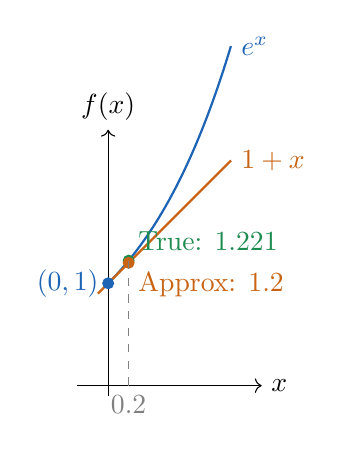
\begin{tikzpicture}[scale=1.3]
  % Axes
  \draw[->] (-0.3,0) -- (1.5,0) node[right] {$x$};
  \draw[->] (0,-0.1) -- (0,2.5) node[above] {$f(x)$};
  % True function
  \draw[thick, ekfblue, domain=0:1.2, samples=60]
    plot (\x, {exp(\x)}) node[right] {$e^x$};
  % Tangent line
  \draw[thick, ekforange, domain=-0.1:1.2]
    plot (\x, {1 + \x}) node[right] {$1 + x$};
  % Points
  \filldraw[ekfblue] (0,1) circle (1.5pt) node[left] {$(0,1)$};
  \filldraw[ekfgreen] (0.2,{exp(0.2)}) circle (1.5pt)
    node[above right] {True: $1.221$};
  \filldraw[ekforange] (0.2,1.2) circle (1.5pt)
    node[below right] {Approx: $1.2$};
  % vertical dashed
  \draw[dashed, gray] (0.2,0) node[below] {$0.2$} -- (0.2,{exp(0.2)});
\end{tikzpicture}
\caption{First-order Taylor approximation of $e^x$ around $x=0$.
         The orange tangent line closely follows the blue true curve near
         the expansion point.}
\label{fig:taylor}
\end{figure}

\subsection{Extension to Multiple Variables — the Jacobian}

For a vector function $f: \mathbb{R}^n \to \mathbb{R}^m$, the scalar
derivative $f'(a)$ generalises to the \textbf{Jacobian matrix}
$\bF_c \in \mathbb{R}^{m \times n}$:

\begin{equation}
  [\bF_c]_{ij} = \frac{\partial f_i}{\partial x_j}\bigg|_{\hat{\bx}}
\end{equation}

The first-order Taylor approximation becomes:
\begin{equation}
  f(\bx) \approx f(\hat{\bx}) + \bF_c\,(\bx - \hat{\bx})
\end{equation}

This is linear in $\bx$.  a Gaussian input $\bx$ produces a Gaussian output,
which is the property the EKF requires.

% ══════════════════════════════════════════════════════════════════════════════
\section{State Transition Jacobian Derivation}
\label{app:State-Transition-Jacobian}

We start from the predicted mean, Equation~\eqref{eq:predict_mean_2}. To
linearise it, first separate the time step from the kinematics by writing
$f(\hat{\bx}_k) = \Delta t\, g(\hat{\bx}_k)$, where
\begin{equation}
  g(\hat{\bx}_k) =
  \begin{bmatrix}
    \bG(\phi,\theta)\,\bomega_c \\
    \bm{0}_3
  \end{bmatrix}
\end{equation}
is the underlying kinematic function, with $\Delta t$ pulled out as an
explicit constant factor. Applying the first-order Taylor expansion of
Equation~\eqref{eq:taylor} to $g$ around the previous state estimate
$\hat{\bx}$ gives:
\begin{equation}
  g(\hat{\bx}_k) \approx g(\hat{\bx}) + \bF_c\,(\hat{\bx}_k - \hat{\bx})
\end{equation}
where $\bF_c = \partial g/\partial \bx|_{\hat{\bx}}$ is exactly the Jacobian
of Equation~\eqref{eq:Fc}.

Substituting $f(\hat{\bx}_k) = \Delta t\, g(\hat{\bx}_k)$ into
Equation~\eqref{eq:predict_mean_2}:
\begin{equation}
  \hat{\bx}_{k+1} = \hat{\bx}_k + \Delta t\, g(\hat{\bx})
                    + \Delta t\,\bF_c\,(\hat{\bx}_k - \hat{\bx})
  \label{eq:predict_mean_3}
\end{equation}
Expanding and grouping every term that multiplies $\hat{\bx}_k$:
\begin{equation}
  \hat{\bx}_{k+1} = (\bI + \Delta t\,\bF_c)\,\hat{\bx}_k
                    + \big[\Delta t\, g(\hat{\bx}) - \Delta t\,\bF_c\,\hat{\bx}\big]
  \label{eq:g_expand}
\end{equation}
The bracketed term does not depend on $\hat{\bx}_k$, so it is a constant
with respect to the random variable $\hat{\bx}_k$. Equation~\eqref{eq:g_expand}
therefore has exactly the form $\hat{\bx}_{k+1} = \bF_d\,\hat{\bx}_k + \bm{c}$,
with $\bF_d = \bI + \Delta t\,\bF_c$ matching Equation~\eqref{eq:Fd}, and
$\bm{c}$ a constant vector.

\subsection{Constants do not affect covariance}

For any random variable $x$ with mean $m$, and any constant $c$, let
$y = x + c$. Then:
\begin{align}
  E[y] &= E[x + c] = E[x] + c = m + c \\
  \mathrm{Cov}(y) &= E\big[(y - E[y])(y - E[y])^\top\big] \notag \\
                   &= E\big[((x+c) - (m+c))((x+c) - (m+c))^\top\big] \notag \\
                   &= E\big[(x-m)(x-m)^\top\big] = \mathrm{Cov}(x)
\end{align}
A constant shifts the mean but leaves the covariance unchanged. Applied to
Equation~\eqref{eq:g_expand}, this means the constant bracketed term
contributes nothing to $\mathrm{Cov}(\hat{\bx}_{k+1})$; only the
$\bF_d\,\hat{\bx}_k$ part matters for covariance propagation.

\subsection{Covariance under a linear transform (the sandwich formula)}
\label{app:sandwich_formula}
Let $\bx$ be a random vector with mean $\mathbf{M}$ and covariance
$\bP = E[(\bx-\mathbf{M})(\bx-\mathbf{M})^\top]$, and let $\mathbf{A}$ be
a constant matrix. Define $\mathbf{y} = \mathbf{A}\bx$. Then:
\begin{align}
  E[\mathbf{y}] &= E[\mathbf{A}\bx] = \mathbf{A}\,E[\bx] = \mathbf{A}\mathbf{M} \\
  \mathrm{Cov}(\mathbf{y}) &= E\big[(\mathbf{A}\bx - \mathbf{A}\mathbf{M})(\mathbf{A}\bx - \mathbf{A}\mathbf{M})^\top\big] \notag \\
                     &= E\big[\mathbf{A}(\bx-\mathbf{M})(\bx-\mathbf{M})^\top \mathbf{A}^\top\big]
                        \qquad \text{using } (\mathbf{A}\mathbf{v})^\top = \mathbf{v}^\top\mathbf{A}^\top \notag \\
                     &= \mathbf{A}\,E\big[(\bx-\mathbf{M})(\bx-\mathbf{M})^\top\big]\,\mathbf{A}^\top
                        = \mathbf{A}\bP\mathbf{A}^\top
\end{align}

\subsection{Result}

Combining both results with $\mathbf{A} = \bF_d$: the constant term in
Equation~\eqref{eq:g_expand} does not affect the covariance, and the
remaining linear term propagates covariance as $\bF_d\bP_k\bF_d^\top$.
This is exactly the first term of Equation~\eqref{eq:predict_cov}; the
additional $\bQ$ term accounts separately for the process noise injected
at each step, which is not part of this deterministic linearisation
argument.

\section{Explicit Entries of the Jacobian \texorpdfstring{$\bF_c$}{Fc}}
\label{app:Fc-entries}

This appendix derives the explicit, fully worked-out entries of
$\bF_c = \partial g/\partial \bx|_{\hat{\bx}}$ (Equation~\eqref{eq:Fc}),
by taking the ordinary partial derivative of each component of
$g(\hat{\bx}_k)$ with respect to each of the six state variables. These
are the exact expressions implemented in software.

\subsection{Expanding \texorpdfstring{$g(\hat{\bx}_k)$}{g}}

Written out fully, $g$ is six equations, one per state variable:
\begin{align}
  \dot\phi   &= \omega_{cx} + \omega_{cy}\sin\phi\tan\theta + \omega_{cz}\cos\phi\tan\theta \notag\\
  \dot\theta &= \omega_{cy}\cos\phi - \omega_{cz}\sin\phi \notag\\
  \dot\psi   &= \omega_{cy}\dfrac{\sin\phi}{\cos\theta} + \omega_{cz}\dfrac{\cos\phi}{\cos\theta} \notag\\
  \dot{b}_x  &= 0 \notag\\
  \dot{b}_y  &= 0 \notag\\
  \dot{b}_z  &= 0
  \label{eq:g-expanded}
\end{align}
The last three equations are simply the constant zero, since the bias
states have no dynamics of their own (Section~\ref{sec:predict}): the
gyroscope bias is modelled as a random walk, so its predicted rate of
change is exactly zero.

\subsection{The Jacobian, in general form}

$\bF_c$ is the matrix of partial derivatives of the six equations in
Equation~\eqref{eq:g-expanded} with respect to the six state variables.
Row $i$ corresponds to the equation being differentiated; column $j$
corresponds to the variable it is differentiated with respect to:
\begin{equation}
  \bF_c =
  \begin{bmatrix}
    \dfrac{\partial \dot\phi}{\partial \phi}   & \dfrac{\partial \dot\phi}{\partial \theta}   & \dfrac{\partial \dot\phi}{\partial \psi}   & \dfrac{\partial \dot\phi}{\partial b_x}   & \dfrac{\partial \dot\phi}{\partial b_y}   & \dfrac{\partial \dot\phi}{\partial b_z}   \\[6pt]
    \dfrac{\partial \dot\theta}{\partial \phi} & \dfrac{\partial \dot\theta}{\partial \theta} & \dfrac{\partial \dot\theta}{\partial \psi} & \dfrac{\partial \dot\theta}{\partial b_x} & \dfrac{\partial \dot\theta}{\partial b_y} & \dfrac{\partial \dot\theta}{\partial b_z} \\[6pt]
    \dfrac{\partial \dot\psi}{\partial \phi}   & \dfrac{\partial \dot\psi}{\partial \theta}   & \dfrac{\partial \dot\psi}{\partial \psi}   & \dfrac{\partial \dot\psi}{\partial b_x}   & \dfrac{\partial \dot\psi}{\partial b_y}   & \dfrac{\partial \dot\psi}{\partial b_z}   \\[6pt]
    \dfrac{\partial \dot{b}_x}{\partial \phi}  & \dfrac{\partial \dot{b}_x}{\partial \theta}  & \dfrac{\partial \dot{b}_x}{\partial \psi}  & \dfrac{\partial \dot{b}_x}{\partial b_x}  & \dfrac{\partial \dot{b}_x}{\partial b_y}  & \dfrac{\partial \dot{b}_x}{\partial b_z}  \\[6pt]
    \dfrac{\partial \dot{b}_y}{\partial \phi}  & \dfrac{\partial \dot{b}_y}{\partial \theta}  & \dfrac{\partial \dot{b}_y}{\partial \psi}  & \dfrac{\partial \dot{b}_y}{\partial b_x}  & \dfrac{\partial \dot{b}_y}{\partial b_y}  & \dfrac{\partial \dot{b}_y}{\partial b_z}  \\[6pt]
    \dfrac{\partial \dot{b}_z}{\partial \phi}  & \dfrac{\partial \dot{b}_z}{\partial \theta}  & \dfrac{\partial \dot{b}_z}{\partial \psi}  & \dfrac{\partial \dot{b}_z}{\partial b_x}  & \dfrac{\partial \dot{b}_z}{\partial b_y}  & \dfrac{\partial \dot{b}_z}{\partial b_z}
  \end{bmatrix}
  \label{eq:Fc-generic}
\end{equation}

\subsection{Rows 4 to 6: the bias rows}

Since $\dot{b}_x, \dot{b}_y, \dot{b}_z$ are each identically zero
(Equation~\eqref{eq:g-expanded}), and the derivative of a constant is
zero with respect to every variable, every entry in the bottom three
rows is zero, regardless of column:
\begin{equation}
  \frac{\partial \dot{b}_x}{\partial \phi} = \frac{\partial \dot{b}_x}{\partial \theta} = \cdots = \frac{\partial \dot{b}_z}{\partial b_z} = 0
\end{equation}

\subsection{Rows 1 to 3, columns 4 to 6: the bias enters through \texorpdfstring{$\bomega_c$}{wc}}

$\bomega_c = \bomega_{\text{meas}} - \hat{\bm{b}}$ is linear in the bias,
and $\bG(\phi,\theta)$ does not depend on it, so:
\begin{equation}
  \frac{\partial(\bG\bomega_c)}{\partial \hat{\bm{b}}}
  = \bG\,\frac{\partial \bomega_c}{\partial \hat{\bm{b}}}
  = \bG \cdot (-\bI_3) = -\bG(\phi,\theta)
\end{equation}
giving the top-right $3\times 3$ block directly.

\subsection{Rows 1 to 3, columns 1 to 3: the remaining derivatives}

Since neither $\bG$ nor $\bomega_c$ depends on $\psi$, the third column
of this block is zero:
\begin{equation}
  \frac{\partial \dot\phi}{\partial \psi} = \frac{\partial \dot\theta}{\partial \psi} = \frac{\partial \dot\psi}{\partial \psi} = 0
\end{equation}
$\dot\theta$ does not depend on $\theta$ either:
\begin{equation}
  \frac{\partial \dot\theta}{\partial \theta} = 0
\end{equation}
The five remaining, nonzero entries are:
\begin{align}
  \frac{\partial \dot\phi}{\partial \phi} &=
    \omega_{cy}\cos\phi\tan\theta - \omega_{cz}\sin\phi\tan\theta \\
  \frac{\partial \dot\phi}{\partial \theta} &=
    \omega_{cy}\sin\phi\sec^2\theta + \omega_{cz}\cos\phi\sec^2\theta \\
  \frac{\partial \dot\theta}{\partial \phi} &=
    -\omega_{cy}\sin\phi - \omega_{cz}\cos\phi \\
  \frac{\partial \dot\psi}{\partial \phi} &=
    \omega_{cy}\cos\phi\sec\theta - \omega_{cz}\sin\phi\sec\theta \\
  \frac{\partial \dot\psi}{\partial \theta} &=
    \omega_{cy}\sin\phi\sec\theta\tan\theta + \omega_{cz}\cos\phi\sec\theta\tan\theta
\end{align}

\subsection{Assembled matrix}

\begin{equation}
  \bF_c =
  \begin{bmatrix}
    \dfrac{\partial \dot\phi}{\partial \phi} & \dfrac{\partial \dot\phi}{\partial \theta} & 0 & -1 & -\sin\phi\tan\theta & -\cos\phi\tan\theta \\[4pt]
    \dfrac{\partial \dot\theta}{\partial \phi} & 0 & 0 & 0 & -\cos\phi & \sin\phi \\[4pt]
    \dfrac{\partial \dot\psi}{\partial \phi} & \dfrac{\partial \dot\psi}{\partial \theta} & 0 & 0 & -\dfrac{\sin\phi}{\cos\theta} & -\dfrac{\cos\phi}{\cos\theta} \\[4pt]
    0 & 0 & 0 & 0 & 0 & 0 \\
    0 & 0 & 0 & 0 & 0 & 0 \\
    0 & 0 & 0 & 0 & 0 & 0
  \end{bmatrix}
  \label{eq:Fc-explicit}
\end{equation}
with the five nonzero top-left entries as derived above. These are the
exact expressions used in the software implementation of the filter.

\section{Explicit Entries of the Jacobian \texorpdfstring{$\bm{H}_m$}{Hm}}
\label{app:Hm-entries}

This appendix derives the explicit entries of
$\bm{H}_m = \partial\bm{h}_m/\partial\bx$ (Equation~\eqref{eq:hm}), by
taking the ordinary partial derivative of each row with respect to
each of the six state variables, the same technique used for $\bm{F}_c$
in Appendix~\ref{app:Fc-entries}. These are the exact expressions
implemented in software.

\subsection{Why columns 4--6 are zero}

$\bm{h}_m(\bx)$, as given in Equation~\eqref{eq:hm}, depends only on
$\phi$, $\theta$, and $\psi$; it does not contain $b_x$, $b_y$, or
$b_z$ at all. The magnetometer measures the orientation of the Earth's
field relative to the body frame, which has no dependence on the
gyroscope's bias. The partial derivative of $\bm{h}_m$ with respect to
each bias component is therefore identically zero, giving the three
zero columns.

\subsection{The nine entries}

Differentiating each row of Equation~\eqref{eq:hm} with respect to
$\phi$, $\theta$, and $\psi$ in turn:

\begin{align}
  \frac{\partial m_{bx}}{\partial \phi} &= 0 \\
  \frac{\partial m_{bx}}{\partial \theta} &= -m_D\cos\theta - m_N\sin\theta\cos\psi \\
  \frac{\partial m_{bx}}{\partial \psi} &= -m_N\sin\psi\cos\theta \\[8pt]
  \frac{\partial m_{by}}{\partial \phi} &= m_D\cos\phi\cos\theta + m_N(\sin\phi\sin\psi + \sin\theta\cos\phi\cos\psi) \\
  \frac{\partial m_{by}}{\partial \theta} &= (m_N\cos\psi\cos\theta - m_D\sin\theta)\sin\phi \\
  \frac{\partial m_{by}}{\partial \psi} &= -m_N(\sin\phi\sin\psi\sin\theta + \cos\phi\cos\psi) \\[8pt]
  \frac{\partial m_{bz}}{\partial \phi} &= -m_D\sin\phi\cos\theta - m_N\sin\phi\sin\theta\cos\psi + m_N\sin\psi\cos\phi \\
  \frac{\partial m_{bz}}{\partial \theta} &= (m_N\cos\psi\cos\theta - m_D\sin\theta)\cos\phi \\
  \frac{\partial m_{bz}}{\partial \psi} &= m_N(\sin\phi\cos\psi - \sin\psi\sin\theta\cos\phi)
\end{align}
Note $\partial m_{bx}/\partial \phi = 0$: the first row of $\bm{h}_m$
does not depend on $\phi$ at all.

\subsection{Assembled matrix}

\begin{equation}
  \bm{H}_m =
  \begin{bmatrix}
    \dfrac{\partial m_{bx}}{\partial \phi} & \dfrac{\partial m_{bx}}{\partial \theta} & \dfrac{\partial m_{bx}}{\partial \psi} & 0 & 0 & 0 \\[8pt]
    \dfrac{\partial m_{by}}{\partial \phi} & \dfrac{\partial m_{by}}{\partial \theta} & \dfrac{\partial m_{by}}{\partial \psi} & 0 & 0 & 0 \\[8pt]
    \dfrac{\partial m_{bz}}{\partial \phi} & \dfrac{\partial m_{bz}}{\partial \theta} & \dfrac{\partial m_{bz}}{\partial \psi} & 0 & 0 & 0
  \end{bmatrix}
  \label{eq:Hm-explicit}
\end{equation}
with the nine entries above substituted in. These are the exact
expressions used in the software implementation of the filter.


\section{Derivation of the Joseph Form}
\label{app:joseph}

The real measurement includes additive noise:
\begin{equation}
  \bm{y} = \bm{H}\bx + \bm{v}, \qquad \bm{v} \sim \mathcal{N}(\bm{0}, \bm{R})
\end{equation}
The state error after the update is:
\begin{align}
  \bx - \hat{\bx}_{\text{new}}
  &= \bx - \hat{\bx} - \bm{K}(\bm{H}(\bx-\hat{\bx}) + \bm{v}) \notag\\
  &= (\bI - \bm{K}\bm{H})(\bx - \hat{\bx}) - \bm{K}\bm{v}
\end{align}
Taking the covariance (cross-terms vanish because state error and
measurement noise $\bm{v}$ are independent):
\begin{align}
  \bP_{\text{new}}
  &= \E\!\left[(\bI{-}\bm{K}\bm{H})(\bx{-}\hat{\bx})(\bx{-}\hat{\bx})^{\top}
    (\bI{-}\bm{K}\bm{H})^{\top}\right]
    + \E\!\left[\bm{K}\bm{v}\bm{v}^{\top}\bm{K}^{\top}\right] \notag\\
  &= (\bI-\bm{K}\bm{H})\,\bP\,(\bI-\bm{K}\bm{H})^{\top}
    + \bm{K}\bm{R}\bm{K}^{\top}
\end{align}
which is Equation~\eqref{eq:joseph}. Both terms are of the form
$\bm{A}\bm{M}\bm{A}^\top$ for a positive-semi-definite $\bm{M}$
($\bP$ and $\bm{R}$ respectively), which is guaranteed
positive-semi-definite for \emph{any} matrix $\bm{A}$
\cite{grewal2015kalman}, including the case where $\bm{K}$ deviates
slightly from the true optimal gain. The simplified form,
$\bP_{\text{new}} = (\bI-\bm{K}\bm{H})\bP$, relies instead on an exact
algebraic cancellation that only holds when $\bm{K}$ is precisely
optimal, and offers no such structural guarantee.


\section{Derivation of the Euler Angle Initial Uncertainty}
\label{app:P0-angle-derivation}

$\theta_0$ and $\phi_0$ are computed from the averaged stationary
accelerometer reading via (Section~\ref{sec:init}):
\begin{equation}
  \theta_0 = \operatorname{atan2}\!\left(-\bar{a}_x,\ \sqrt{\bar{a}_y^2+\bar{a}_z^2}\right),
  \qquad
  \phi_0 = \operatorname{atan2}(\bar{a}_y,\ \bar{a}_z)
\end{equation}

\subsection{Jacobian of the inversion}

The Jacobian of this transformation with respect to
$[\bar{a}_x,\bar{a}_y,\bar{a}_z]$, substituting the gravity model
relationship $\bar{a}_x=-g\sin\theta$, $\bar{a}_y=g\sin\phi\cos\theta$,
$\bar{a}_z=g\cos\phi\cos\theta$ and evaluated at a level device
($\phi=0$, $\theta=0$), simplifies to:
\begin{equation}
  \bm{J} = \frac{\partial[\theta_0,\phi_0]}{\partial[\bar{a}_x,\bar{a}_y,\bar{a}_z]}
  \bigg|_{\phi=0,\theta=0}
  = \begin{bmatrix} -\dfrac{1}{g} & 0 & 0 \\[6pt] 0 & \dfrac{1}{g} & 0 \end{bmatrix}
  \label{eq:J_angle_init}
\end{equation}
matching the intuitive small-angle result: near level, $\bar{a}_x
\approx -g\theta$ and $\bar{a}_y \approx g\phi$, so
$\theta \approx -\bar{a}_x/g$ and $\phi \approx \bar{a}_y/g$ directly.

\subsection{Covariance of the averaged reading}

Since $\bar{a}_x, \bar{a}_y, \bar{a}_z$ are each the mean of $N$
independent stationary samples with per-axis sensor noise $\sigma_a$
(Section~\ref{sec:noise-characterization}), their covariance is:
\begin{equation}
  \bm{P}_{\bar{a}} = \operatorname{diag}\!\left(\frac{\sigma_{ax}^2}{N},\ \frac{\sigma_{ay}^2}{N},\ \frac{\sigma_{az}^2}{N}\right)
\end{equation}

\subsection{Propagating through the Jacobian}

Applying the same covariance sandwich rule used throughout this filter
(Appendix~\ref{app:sandwich_formula}):
\begin{equation}
  \operatorname{Cov}([\theta_0,\phi_0]) = \bm{J}\,\bm{P}_{\bar{a}}\,\bm{J}^\top
  = \begin{bmatrix} \dfrac{\sigma_{ax}^2}{N g^2} & 0 \\[6pt] 0 & \dfrac{\sigma_{ay}^2}{N g^2} \end{bmatrix}
  \label{eq:cov_angle_init}
\end{equation}
giving Equation~\eqref{eq:sigma_theta0_phi0}, with the zero
off-diagonal entries confirming no cross-covariance between $\theta_0$
and $\phi_0$ at this operating point.

%====================
\section{Python Reference Model Source}
\label{app:python-source}

The complete source of the software model, as used for every result
in this thesis. Line references in Chapter~\ref{ch:ekf-design}
point here.

\subsection{\texttt{EKF.py}}
\label{app:ekf-py}
\lstinputlisting[language=Python]{Code/EKF_py_model/EKF.py}

\subsection{\texttt{data\_preparer.py}}
\label{app:data-preparer-py}
\lstinputlisting[language=Python]{Code/EKF_py_model/data_preparer.py}
% ══════════════════════════════════════════════════════════════════════════════
\bibliographystyle{ieeetr}   % or plain, unsrt, apalike, etc.
\bibliography{references}    % no .bib extension here

\end{document}


\end{document}


